
\chapter{Introduction and notation}
\label{ch:intro}

{\em Wisdom is the quality that keeps you from getting into situations where you need it.  --Doug Larson}

\section{Basic sets}
\label{sec:basic}

It has been said\index{Kronecker, Leopold}\footnote{Usually attributed to 
Kronecker -- ``Die ganze Zahl schuf der liebe Gott, alles \"{U}brige 
ist Menschenwerk.''} that ``God invented
the integers, all else is the work of Man.''  This is 
a mistranslation.  The term ``integers'' should
actually be ``whole numbers.''  The concepts of zero and negative 
values seem (to many people) to be unnatural constructs.  Indeed, otherwise
intelligent people are still known to rail against the concept of a
negative quantity -- ``How can you have negative three apples?'' 
The concept of zero is also somewhat profound.

Probably most people will agree that the 
\index{natural numbers} natural numbers {\em are} a natural construct -- they are the numbers we use to count things.  Traditionally, the natural numbers are denoted $\Naturals$.

At this point in time there seems to be no general agreement about the status
of zero ($0$) as a natural number.  Are there collections that we might possibly
count that have \emph{no} members?  Well, yes -- I'd invite you to consider the collection of gold bars that I keep in my basement\ldots

The traditional view seems to be that 

\[ \Naturals = \{1, 2, 3, 4, \ldots \} \]

\noindent i.e.\ that the naturals don't include 0.  My personal 
preference would be to make the other choice (i.e.\ to include $0$
in the natural numbers), but for the moment, let's be traditionalists.

\noindent Be advised that this is a choice.  We are adopting a 
convention.  If in some other course, or other mathematical setting 
you find that the other convention is preferred, well, it's good to
learn flexibility\ldots

Perhaps the best way of saying what a set is, is to do as we 
have above.  List all the elements.  Of course, if a set has an
infinite number of things in it, this is a difficult task -- so
we satisfy ourselves by listing enough of the elements that the
pattern becomes clear.

Taking $\Naturals$ for granted, what is meant by the ``all else''
that humankind is responsible for?  The basic sets of different types
of ``numbers'' that every mathematics student should know are: $\Naturals,
\Integers, \Rationals, \Reals
\; \mbox{and} \; \Complexes$.  Respectively: the naturals, the integers, the
rationals, the reals, and the complex numbers.  The use of $\Naturals,
\Reals \; \mbox{and} \; \Complexes$ is probably clear to an English
speaker.  The integers are denoted with a $\Integers$ because of the
German word {\em z\"{a}hlen} which means ``to count.''   The rational numbers are
probably denoted using $\Rationals$, for ``quotients.''  Etymology
aside, is it possible for us to provide precise descriptions of these
remaining sets?  

The \index{integers} integers ($\Integers$) are just the set of natural numbers
together with the negatives of naturals and zero.  We can use
a doubly infinite list to denote this set.

\[ \Integers = \{ \ldots -3, -2, -1, 0, 1, 2, 3, \ldots \} \]


To describe the \index{rationals} rational numbers precisely we'll have to wait until Section~\ref{sec:rat}.
In the interim, we can use an intuitively appealing, but somewhat imprecise
definition for the set of rationals.  A rational number is a fraction built out
of integers.   This also provides us with
a chance to give an example of using the main other way of describing
the contents of a set -- so-called \index{set-builder notation} set-builder notation.

\[ \Rationals = \{ \frac{a}{b} \suchthat a \in \Integers \; \mbox{and} \;
b \in \Integers \; \mbox{and} \; b \neq 0 \} \]

This is a good time to start building a ``glossary'' -- a translation lexicon
between the symbols of mathematics and plain language.  In the line
above we are defining the set $\Rationals$ of rational numbers, so the
first symbols that appear are ``$\Rationals =$.''  It is interesting to 
note that the equals sign has two subtly different meanings: assignment
and equality testing,  in the mathematical sentence above we are
making an assignment -- that is, we are declaring that from now on the set
$\Rationals$ will {\em be} the set defined on the remainder of the
line.\footnote{Some Mathematicians contend that only the ``equality
  test'' meaning of the equals sign is real, that by writing the
  mathematical sentence above we are asserting the truth of the
  equality test.  This may be technically correct but it isn't how
  most people think of things.}  
Let's dissect the rest of that line now.  There are only 4 
characters whose meaning may be in doubt, $\{$, $\}$, $\in$ and $\suchthat$.
The curly braces (a.k.a. {\em french braces}) are almost universally
reserved to denote sets, anything appearing between curly braces is 
meant to define a set.  In translating from ``math'' to English,
replace the initial brace with the phrase ``the set of all.''  The 
next arcane symbol to appear is the vertical bar.  As we will see in
Section~\ref{div} this symbol has (at least) two meanings -- it will
always be clear from context which is meant.  In the sentence we are
analyzing, it stands for the words ``such that.''  The last bit of
arcana to be deciphered is the symbol $\in$, it stands for the English
word ``in'' or, more formally, ``is an element of.''

Let's parse the entire mathematical sentence we've been discussing
with an English translation in parallel.

\vspace{.2in}

\begin{tabular}{c|c|c}
\rule[-10pt]{0pt}{22pt} $\Rationals$ & $=$ & $\{$  \\ \hline
\rule[-6pt]{0pt}{22pt} The rational numbers & are defined to be & the set of all\\
\end{tabular}

\vspace{.2in}

\begin{tabular}{c|c}
\rule[-10pt]{0pt}{22pt} $\displaystyle \frac{a}{b}$ & $\suchthat$ \\ \hline
\rule[-6pt]{0pt}{22pt} fractions of the form $a$ over $b$ & such that \\
\end{tabular}

\vspace{.2in}

\begin{tabular}{c|c|c}
\rule[-10pt]{0pt}{22pt} $a \in \Integers$ & and & $b \in \Integers$ \\ \hline
\rule[-6pt]{0pt}{22pt} $a$ is an element of the integers & and & $b$ is an
element of the integers \\
\end{tabular}

\vspace{.2in}

\begin{tabular}{c|c|c}
\rule[-10pt]{0pt}{22pt} and & $b \neq 0$ & $\}$ \\ \hline
\rule[-6pt]{0pt}{22pt} and & $b$ is nonzero. & (the final curly brace
is silent) \\
\end{tabular}

\vspace{.2in}

It is quite apparent that the mathematical notation represents a huge
improvement as regards brevity. 

As mentioned previously, this definition is slightly flawed.  We will
have to wait 'til later to get a truly precise
definition of the rationals, but we invite the reader to mull over
what's wrong with this one.  Hint: think about the issue of whether
a fraction is in lowest terms.

Let's proceed with our menagerie of sets of numbers.  The next set
we'll consider is $\Reals$, the set of\index{reals} real numbers.  To someone
who has completed Calculus, the reals are perhaps the most obvious and
natural notion of what is meant by ``number.''  It may be surprising to
learn that the actual definition of what is meant by a real number is
extremely difficult.  In fact, the first reasonable formulation of a
precise definition of the reals came around 1858, more than 180 years
after the development of the 
Calculus\index{Newton, Isaac}\footnote{Although it was not
  published until 1736, Newton's book (De Methodis Serierum et
  Fluxionum) describing both differential and integral Calculus was
  written in 1671.}.  A precise 
definition for the set $\Reals$ of real numbers is 
beyond the scope of this book, for the moment consider the
following intuitive description.  A real number is a number that 
measures some physical quantity.  For example, if a circle has
diameter 1 then its circumference is $\pi$, thus $\pi$ is a real
number.  The points $(0,0)$ and $(1,1)$ in the Cartesian plane have
distance $\sqrt{ (0-1)^2 + (0-1)^2} = \sqrt{2}$, thus $\sqrt{2}$ is 
a real number.  Any rational number is clearly a real number -- slope
is a physical quantity, and the line from $(0,0)$ to $(b,a)$ has slope
$a/b$.  In ancient Greece, \index{Pythagoras}Pythagoras -- who has sometimes been
described as the first pure Mathematician, believed that 
every real quantity was in fact rational, a belief that we now know to
be false.  The numbers $\pi$ and $\sqrt{2}$ mentioned above are not
rational numbers.  For the moment it is useful to recall a practical
method for distinguishing between rational numbers and real quantities
that are not rational -- consider their decimal expansions.  If the
reader is unfamiliar with the result to which we are alluding, we urge
you to experiment.  Use a calculator or (even better) a computer
algebra package to find the decimal expansions of various quantities.
Try $\pi$, $\sqrt{2}$, $1/7$, $2/5$, $16/17$, $1/2$ and a few other
quantities of your own choice.  Given that we have already said that the first
two of these are not rational, try to determine the pattern.  What is 
it about the decimal expansions
that distinguishes rational quantities from reals that aren't rational?

Given that we can't give a precise definition of a real number at this
point it is perhaps surprising that we {\em can} define the set
$\Complexes$ of \index{complex numbers}complex numbers with precision 
(modulo the fact that we define them in terms of $\Reals$).  

\[ \Complexes = \{ a + bi \suchthat a \in \Reals \; \mbox{and} \; b \in
\Reals \; \mbox{and} \; i^2 = -1 \} \]

Translating this bit of mathematics into English we get: 

\vspace{.2in}

\begin{tabular}{c|c|c}
\rule[-10pt]{0pt}{22pt} $\Complexes$ & $=$ & $\{$  \\ \hline
\rule[-6pt]{0pt}{22pt} The complex numbers & are defined to be & the set of all\\
\end{tabular}

\vspace{.2in}

\begin{tabular}{c|c}
\rule[-10pt]{0pt}{22pt} $a+bi$ & $\suchthat$ \\ \hline
\rule[-6pt]{0pt}{22pt} expressions of the form $a$ plus $b$ times $i$ & such that \\
\end{tabular}

\vspace{.2in}

\begin{tabular}{c|c|c}
\rule[-10pt]{0pt}{22pt} $a \in \Reals$ & and & $b \in \Reals$ \\ \hline
\rule[-6pt]{0pt}{22pt} $a$ is an element of the reals & and & $b$ is an
element of the reals \\
\end{tabular}

\vspace{.2in}

\begin{tabular}{c|c|c}
\rule[-10pt]{0pt}{22pt} and & $i^2 = -1$ & $\}$ \\ \hline
\rule[-6pt]{0pt}{22pt} and & $i$ has the property that its
square is negative one. &  \\
\end{tabular}

\vspace{.2in}

We sometimes denote a complex number using a single variable (by
convention, either late alphabet Roman letters or Greek letters.
Suppose that we've defined $z = a + bi$.  The single letter $z$
denotes the entire complex number.  We can extract the individual
components of this complex number by talking about the 
\index{real part}real and
\index{imaginary part}imaginary parts of $z$.  
Specifically, $Re(z) = a$ is called the
real part of $z$, and $Im(z) = b$ is called the imaginary part of
$z$.


Complex numbers are added and multiplied as if they were binomials
(polynomials with just two terms) where $i$ is treated as if it were 
the variable -- except that we use the algebraic property that $i$'s
square is -1.  For example, to add the complex numbers $1+2i$ and
$3-6i$ we just think of the binomials $1+2x$ and $3-6x$.  Of course we
normally write a binomial with the term involving the variable coming
first, but this is just a convention.  The sum of those binomials
would be $4-4x$ and so the sum of the given complex numbers is $4-4i$.
This sort of operation is fairly typical and is called 
\index{component-wise operations}{\em  component-wise} addition.  
To multiply complex numbers we have to
recall how it is that we multiply binomials.  This is the well-known
FOIL rule (first, outer, inner, last).  For example the product of
$3-2x$ and $4+3x$ is $(3\cdot 4) + (3 \cdot 3x) + (-2x\cdot 4) +
(-2x\cdot 3x)$ this expression simplifies to $12 + x - 6x^2$.  The
analogous calculation with complex numbers looks just the same, until
we get to the very last stage where, in simplifying, we use the fact
that $i^2=-1$.  

\begin{gather*}
 (3-2i)\cdot (4+3i) \\
= (3\cdot 4) + (3\cdot 3i) + (-2i\cdot 4) + (-2i\cdot 3i) \\
= 12 + 9i - 8i -6i^2 \\
= 12 + i + 6 \\
= 18 + i 
\end{gather*}


The real numbers have a natural ordering, and hence, so do the 
other sets that are contained in $\Reals$.  The complex numbers 
can't really be put into a well-defined order --- which should be
bigger, $1$  or $i$?  But we do have a way to, at least partially, 
accomplish this task.  The \index{modulus, of a complex number}
\emph{modulus} of a complex number is a real number that gives the
distance from the origin ($0+0i$) of the complex plane, to a given
complex number.  We indicate the modulus using absolute value bars,
and you should note that if a complex number happens to be purely
real, the modulus and the usual notion of absolute value coincide.
If $z = a + bi$ is a complex number, then its modulus, $\|a + bi \|$,
is given by the formula $\sqrt{a^2+b^2}$.  

Several of the sets of numbers we've been discussing can be split
up based on the so-called \index{trichotomy}\emph{trichotomy property}:
every real number is either positive, negative or zero.  In particular,
$\Integers$, $\Rationals$ and $\Reals$ can have modifiers stuck on so
that we can discuss (for example) the negative real numbers, or the
positive rational numbers or the integers that aren't negative.  
To do this, we put superscripts on the set symbols, either a $+$ 
or a $-$ or the word \index{noneg}``noneg.''

So 

\[ \Integers^+ \; = \; \{ x \in \Integers \suchthat x > 0 \} \]

\noindent and 

\[ \Integers^- \; = \; \{ x \in \Integers \suchthat x < 0 \} \]

\noindent and 

\[ \Znoneg \; = \; 
\{ x \in \Integers \suchthat x \geq 0 \}. \]

Presumably, we could also use ``nonpos'' as a superscript to indicate
non-positive integers, but this never seems to come up in practice.
Also, you should note that $\Integers^+$  is really the same thing
as $\Naturals$, but that  $\Znoneg$  is different because it 
contains $0$.


We would be remiss in closing this section without discussing the
way the sets of numbers we've discussed fit together.  Simply put,
each is contained in the next.  $\Naturals$ is contained in $\Integers$, 
$\Integers$ is contained in $\Rationals$, $\Rationals$ is contained
in $\Reals$, and $\Reals$ is contained in $\Complexes$.
Geometrically the complex numbers are essentially a two-dimensional
plane.  The real numbers sit inside this plane just as the $x$-axis
sits inside the usual Cartesian plane -- in this context you may
hear people talk about ``the real line within the complex plane.''
It is probably clear how $\Naturals$ lies within $\Integers$, and 
every integer is certainly a real number.  The intermediate set
$\Rationals$ (which contains the integers, and is contained by the
reals) has probably the most interesting relationship with the
set that contains it.  Think of the real line as being solid, like
a dark pencil stroke.  The rationals are like sand that has been
sprinkled very evenly over that line.  Every point on the line
 has bits of sand nearby, but not (necessarily) on top of it.


\newpage

\noindent{\large \bf Exercises --- \thesection\ }

\begin{enumerate}

\item Each of the quantities indexing the rows of the following table
is in one or more of the sets which index the columns.  Place a 
check mark in a table entry if the quantity is in the set.

\begin{tabular}{|c||c|c|c|c|c|} \hline
 & $\Naturals$ & $\Integers$ & $\Rationals$ & $\Reals$ & $\Complexes$
 \\ \hline\hline
\rule{0pt}{15pt} $17$ & & & & & \\ \hline
\rule{0pt}{15pt} $\pi$ & & & & & \\ \hline
\rule{0pt}{15pt} $22/7$ & & & & & \\ \hline
\rule{0pt}{15pt} $-6$ & & & & & \\ \hline
\rule{0pt}{15pt} $e^0$ & & & & & \\ \hline
\rule{0pt}{15pt} $1+i$ & & & & & \\ \hline
\rule{0pt}{15pt} $\sqrt{3}$ & & & & & \\ \hline
\rule{0pt}{15pt} $i^2$ & & & & & \\  \hline
\end{tabular}

\hint{Note that these sets contain one another, so if %
you determine that a number is a natural number it is automatically %
an integer and a rational number and a real number and a complex number\ldots}

\vfill

\hintspagebreak
\workbookpagebreak

\item Write the set $\Integers$ of integers using a singly infinite
listing.

\twsvspace{.25in}{1in}{.15in}

\hint{What the heck is meant by a ``singly infinite listing''?  To help you figure this out, note that 
\[ \ldots -3, -2, -1, 0, 1, 2, 3, \ldots \] 
\noindent is a doubly infinite listing.}

\vfill


\item Identify each as rational or irrational.
\begin{enumerate}
\item $5021.2121212121\ldots$
\item $0.2340000000\ldots$
\item $12.31331133311133331111\ldots$
\item $\pi$
\item $2.987654321987654321987654321\ldots$
\end{enumerate}

\vfill

\hint{rat,rat,irr,irr,rat}

\vfill

\textbookpagebreak

\item The ``see and say'' sequence is produced by first writing a 1, 
then iterating the following procedure:  look at the previous entry 
and say how many entries there are of each integer and write down what 
you just said.  The first several terms of the ``see and say'' sequence 
are $1, 11, 21, 1112, 3112, 211213, 312213, 212223, \ldots$.  Comment on the
rationality (or irrationality) of the number whose decimal digits are obtained 
by concatenating the ``see and say'' sequence.

\[ 0.1112111123112211213... \]

\vfill

\hint{
Experiment!

What would it mean for this number to be rational?  If we were to
run into an element of the ``see and say'' sequence that is its own description, then
from that point onward the sequence would get stuck repeating the same thing over and over
(and the number whose digits are found by concatenating the elements of the ``see and say'' 
sequence will enter into a repeating pattern.)
} 
\vfill

\workbookpagebreak

\item Give a description of the set of rational numbers whose decimal
expansions terminate.  (Alternatively, you may think of their decimal
expansions ending in an infinitely-long string of zeros.)

\hint{If a decimal expansion terminates after, say, k digits, can you figure out how to produce an integer from that number? Think about multiplying by something \ldots}

\vfill

\item Find the first 20 decimal places of $\pi$, $3/7$, $\sqrt{2}$, 
  $2/5$, $16/17$, $\sqrt{3}$, $1/2$ and $42/100$.  Classify each of
these quantity's decimal expansion as: terminating, having a repeating
pattern, or showing no discernible pattern.

\hint{A calculator will generally be inadequate for this problem.  You should try using a CAS (Computer Algebra System).  I  would recommend the Sage computer algebra system because
like this book it is free -- you can download sage and run it on your own system or you can try it out online without installing.  Check it out at www.sagemath.org.

You can get sage to output $\pi$ to high accuracy by typing {\tt pi.N(digits=21)}
at the sage$>$ prompt.}

\vfill

\workbookpagebreak
 
\item Consider the process of long division.  Does this algorithm give
any insight as to why rational numbers have terminating or repeating
decimal expansions?  Explain.

\hint{You really need to actually sit down and do some long division problems.  When in the process do you suddenly realize that the digits are going to repeat?  Must this decision point always occur? Why?}

\vfill

\item Give an argument as to why the product of two rational numbers
is again a rational.

\hint{Take for granted that the usual rule for multiplying two fractions is okay to use:

\[ \frac{a}{b} * \frac{c}{d} \; = \; \frac{ac}{bd}. \]

\noindent How do you know that the result is actually a rational number?}

\vfill

\textbookpagebreak

\hintspagebreak

\item Perform the following computations with complex numbers

  \begin{enumerate}
  \item \rule{0pt}{20pt}$ (4 + 3i) - (3 + 2i) $
  \item \rule{0pt}{20pt}$ (1 + i) + (1 - i) $
  \item \rule{0pt}{20pt}$ (1 + i) \cdot (1 - i) $
  \item \rule{0pt}{20pt}$ (2 - 3i) \cdot (3 - 2i) $
  \end{enumerate}

\hint{These are straightforward.  If you really must verify these somehow, you can go to a CAS like Sage, or you can learn how to enter complex numbers on your graphing calculator. (On my TI-84, you get i by hitting the 2nd key and then the decimal point.)
}

\workbookpagebreak

\item The {\em conjugate} of a complex number is denoted with a
  superscript star, and is formed by negating the imaginary part.
  Thus if $z = 3+ 4i$ then the conjugate of $z$ is  $z^\ast = 3-4i$.
  Give an argument as to why the product of a complex number and its
  conjugate is a real quantity.  (I.e.\ the imaginary part of
  $z\cdot z^\ast$ is necessarily 0, no matter what complex number is
  used for $z$.) 

\hint{This is really easy, but be sure to do it generically.  In other words, don't just use examples -- do the calculation with variables for the real and imaginary parts of the complex number.
}

\vfill

\workbookpagebreak

\end{enumerate}



%% Emacs customization
%% 
%% Local Variables: ***
%% TeX-master: "GIAM.tex" ***
%% comment-column:0 ***
%% comment-start: "%% "  ***
%% comment-end:"***" ***
%% End: ***



\newpage

\section{Definitions: Prime numbers}
\label{sec:def}

You may have noticed that in Section~\ref{sec:basic} an awful lot of
emphasis was placed on whether we had good, precise definitions
for things.  Indeed, more than once apologies were made for giving
imprecise or intuitive definitions.  This is because, in Mathematics,
definitions are our lifeblood.  More than in any other human 
endeavor, Mathematicians strive for precision.  This precision
comes with a cost -- Mathematics can deal with only the very 
simplest of phenomena\footnote{For an intriguing discussion of this 
point, read Gian Carlo Rota's book {\em Indiscrete Thoughts}~\cite{rota}.}.  
To laypeople who think of math as being
a horribly difficult subject, that last sentence will certainly 
sound odd, but most professional Mathematicians will be nodding 
their heads at this point.  Hard questions are more properly dealt 
with by Philosophers than by Mathematicians.  Does a cat have 
a soul?  Impossible
to say, because neither of the nouns in that question can be 
defined with any precision.  Is the square root of 2 a rational number?
Absolutely not!  The reason
for the certainty we feel in answering this second question is
that we know {\em precisely} what is meant by the phrases 
``square root of 2'' and ``rational number.''

We often need to first approach
a topic by thinking visually or intuitively, but when it comes to
proving our assertions, nothing beats the power of having the
``right'' definitions around.  It may be surprising to learn that
the ``right'' definition often evolves over the years.  This 
happens for the simple reason that some definitions lend themselves
more easily to proving assertions.  In fact, it is often the case
that definitions are inspired by attempts to prove something that 
fail.  In the midst of such a failure, it isn't uncommon for a 
Mathematician to bemoan ``If only the definition of (fill in the 
blank) were \ldots'', then to realize that it is possible to
use that definition or a modification of it.  But! When there are 
several definitions
for the same idea they had better agree with one another!  

Consider the definition of a \index{prime numbers}prime number. 

\begin{defi} 
A {\em prime number} is a positive integer,
greater than 1, whose only factors are 1 and itself.
\end{defi}

You probably first heard this definition in Middle School, if not
earlier.  It is a perfectly valid definition of what it means 
for an integer to be prime.  In more advanced mathematics, it
was found that it was necessary to define a notion of primality
for objects other than integers.  It turns out that the following
statement is essentially equivalent to the definition of ``prime'' we've just
given (when dealing with integers), but that it can be applied in 
more general settings.

\begin{defi}
A {\em prime} is a quantity $p$ such that whenever $p$ is a 
factor of some product $ab$, then either $p$ is a factor of
$a$ or $p$ is a factor of $b$.
\end{defi}

\begin{exer}
The number 1 is {\em not} considered to be a prime.  Does
1 satisfy the above definition?
\end{exer}

If you go on to study Number Theory or Abstract Algebra you'll see how
the alternate definition we've given needs to be tweaked so that (for example) 
1 \emph{wouldn't} get counted as a prime.  The fix isn't hugely complicated (but it 
is a {\em little} complicated) and is a bit beyond our scope right now\ldots
 
Often, it is the case that we can formulate {\em many} equivalent
definitions for some concept.  When this happens you may run
across the abbreviation \index{TFAE}TFAE, which stands for ``The following
are equivalent.''  A TFAE proof consists of showing that a host
of different statements actually define the same concept.

Since we have been discussing primes in this section (mainly 
as an example of a concept with more than one equivalent 
definition), this seems like a reasonable time to make some
explorations relative to prime numbers.  We'll begin in the 
third century B.C..   \index{Eratosthenes of Cyrene}
Eratosthenes of Cyrene was a Greek Mathematician and
Astronomer who is remembered to this day for his many accomplishments.
He was a librarian at the great library of Alexandria.  He made
measurements of the Earth's circumference and the distances of
the Sun and Moon that were remarkably accurate, but probably his
most remembered achievement is the ``sieve'' method for finding
primes.  Indeed, the \index{sieve of Eratosthenes}sieve of Eratosthenes 
is still of importance
in mathematical research.  Basically, the sieve method consists 
of creating a very long list of natural numbers and then crossing
off all the numbers that aren't primes (a positive integer that
isn't 1, and isn't a prime is called \index{composite}\emph{ composite}).  
This process
is carried out in stages.  First we circle 2 and then cross off
every number that has 2 as a factor -- thus we've identified 
2 as the first prime number and eliminated a whole bunch of numbers 
that aren't prime.  The first number that hasn't been eliminated at
this stage is 3, we circle it (indicating that 3 is the second prime
number) and then cross off every number that has 3 as a factor.  Note
that some numbers (for example, 6 and 12) will have been crossed off
more than once!  In the third stage of the sieve process, we circle
5, which is the smallest number that hasn't yet been crossed off, and
then cross off all multiples of 5.  The first three stages in the
sieve method are shown in Figure~\ref{fig:sieve}.

\begin{figure}[!hbtp]
\input{figures/Eratosthenes.tex}
\caption[The sieve of Eratosthenes.]{The first three stages in the %
sieve of Eratosthenes.  What is the smallest composite number that %
hasn't been crossed off?}
\label{fig:sieve} 
\end{figure}

It is interesting to note that the sieve gives us a means of finding
all the primes up to $p^2$ by using the primes up to (but not
including) $p$.  For
example, to find all the primes less than $13^2 = 169$, we need only
use $2, 3, 5, 7$ and $11$ in the sieve.

Despite the fact that one can find primes using this simple 
mechanical method, the way that prime numbers are distributed
amongst the integers is very erratic.  Nearly any statement that
purports to show some regularity in the distribution of the 
primes will turn out to be false.  Here are two such false
conjectures regarding prime numbers.

\begin{conj} \label{conj:ferm}
Whenever $p$ is a prime number, $2^p-1$ is also a prime.
\end{conj}

\begin{conj} \label{conj:poly}
The polynomial $x^2-31x+257$ evaluates to a prime number
whenever $x$ is a natural number.
\end{conj}

In the exercises for this section, you will be asked to
explore these statements further.  

Prime numbers act as multiplicative building blocks for the rest of
the integers.  When we disassemble an integer into its building blocks
we are finding the \index{prime factorization}\emph{prime factorization} 
of that number.  Prime
factorizations are unique.  That is, a number is either prime or it
has prime factors (possibly raised to various powers) that are
uniquely determined -- except that they may be re-ordered.

On the next page
is a table that contains all the primes that are less than 5000.
Study this table and discover the secret of its compactness!

\newpage


\renewcommand{\tabcolsep}{2.4pt}
\renewcommand{\arraystretch}{.63}
\addtolength{\lineskip}{-2pt}
{\small 
\hspace{-.5in}
\begin{tabular}{|lr|cccc|cccc|cccc|cccc|cccc|cccc|cccc|cccc|cccc|cccc|}
  \hline 
\rule{0pt}{10pt} & \bf T & \multicolumn{4}{c|}{\bf 0} & \multicolumn{4}{c|}{\bf 1} &
 \multicolumn{4}{c|}{\bf 2} & \multicolumn{4}{c|}{\bf 3} & \multicolumn{4}{c|}{\bf 4}
 & \multicolumn{4}{c|}{\bf 5} & \multicolumn{4}{c|}{\bf 6} &
 \multicolumn{4}{c|}{\bf 7} & \multicolumn{4}{c|}{\bf 8} & \multicolumn{4}{c|}{\bf 9}
 \\
\bf H & & & & & & & & & & & & & & & & & & & & & & & & & & & & & & & & & &
 & & & & & & & \\ \hline
\rule{0pt}{9pt}\bf 0 & & 2 & 3 & 5 & 7 & 1 & 3 & 7 & 9 & & 3 & & 9 & 1 & & 7 & & 1 & 3 & 7 & & & 3 & & 9 & 1 & & 7 & & 1 & 3 & & 9 & & 3 & & 9 & & & 7 & \\
\bf 1 & & 1 & 3 & 7 & 9 & & 3 & & & & & 7 & & 1 & & 7 & 9 & & & & 9 & 1 & & 7 & & & 3 & 7 & & & 3 & & 9 & 1 & & & & 1 & 3 & 7 & 9 \\
\bf 2 & & & & & & 1 & & & & & 3 & 7 & 9 & & 3 & & 9 & 1 & & & & 1 & & 7 & & & 3 & & 9 & 1 & & 7 & & 1 & 3 & & & & 3 & & \\
\bf 3 & & & & 7 & & 1 & 3 & 7 & & & & & & 1 & & 7 & & & & 7 & 9 & & 3 & & 9 & & & 7 & & & 3 & & 9 & & 3 & & 9 & & & 7 & \\
\bf 4 & & 1 & & & 9 & & & & 9 & 1 & & & & 1 & 3 & & 9 & & 3 & & 9 & & & 7 &
& 1 & 3 & 7 & & & & & 9 & & & 7 & & 1 & & & 9 \\ \hline
\rule{0pt}{9pt}\bf 5 & & & 3 & & 9 & & & & & 1 & 3 & & & & & & & 1 & & 7 & & & & 7 & & & 3 & & 9 & 1 & & 7 & & & & 7 & & & 3 & & 9 \\
\bf 6 & & 1 & & 7 & & & 3 & 7 & 9 & & & & & 1 & & & & 1 & 3 & 7 & & & 3 & & 9 & 1 & & & & & 3 & 7 & & & 3 & & & 1 & & & \\
\bf 7 & & 1 & & & 9 & & & & 9 & & & 7 & & & 3 & & 9 & & 3 & & & 1 & & 7 & & 1 & & & 9 & & 3 & & & & & 7 & & & & 7 & \\
\bf 8 & & & & & 9 & 1 & & & & 1 & 3 & 7 & 9 & & & & 9 & & & & & & 3 & 7 & 9 & & 3 & & & & & 7 & & 1 & 3 & 7 & & & & & \\
\bf 9 & & & & 7 & & 1 & & & 9 & & & & 9 & & & 7 & & 1 & & 7 & & & 3 & & & &
& 7 & & 1 & & 7 & & & 3 & & & 1 & & 7 & \\ \hline
\rule{0pt}{9pt}\bf 10 & & & & & 9 & & 3 & & 9 & 1 & & & & 1 & 3 & & 9 & & & & 9 & 1 & & & & 1 & 3 & & 9 & & & & & & & 7 & & 1 & 3 & 7 & \\
\bf 11 & & & 3 & & 9 & & & 7 & & & 3 & & 9 & & & & & & & & & 1 & 3 & & & & 3 & & & 1 & & & & 1 & & 7 & & & 3 & & \\
\bf 12 & & 1 & & & & & 3 & 7 & & & 3 & & 9 & 1 & & 7 & & & & & 9 & & & & 9 & & & & & & & 7 & 9 & & 3 & & 9 & 1 & & 7 & \\
\bf 13 & & 1 & 3 & 7 & & & & & 9 & 1 & & 7 & & & & & & & & & & & & & & 1 & & 7 & & & 3 & & & 1 & & & & & & & 9 \\
\bf 14 & & & & & 9 & & & & & & 3 & 7 & 9 & & 3 & & 9 & & & 7 & & 1 & 3 & & 9
& & & & & 1 & & & & 1 & 3 & 7 & 9 & & 3 & & 9 \\ \hline
\rule{0pt}{9pt}\bf 15 & & & & & & 1 & & & & & 3 & & & 1 & & & & & 3 & & 9 & & 3 & & 9 & & & 7 & & 1 & & & 9 & & 3 & & & & & 7 & \\
\bf 16 & & 1 & & 7 & 9 & & 3 & & 9 & 1 & & 7 & & & & 7 & & & & & & & & 7 & & & 3 & 7 & 9 & & & & & & & & & & 3 & 7 & 9 \\
\bf 17 & & & & & 9 & & & & & 1 & 3 & & & & 3 & & & 1 & & 7 & & & 3 & & 9 & & & & & & & 7 & & & 3 & 7 & 9 & & & & \\
\bf 18 & & 1 & & & & 1 & & & & & 3 & & & 1 & & & & & & 7 & & & & & & 1 & & 7 & & 1 & 3 & 7 & 9 & & & & 9 & & & & \\
\bf 19 & & 1 & & 7 & & & 3 & & & & & & & 1 & 3 & & & & & & 9 & 1 & & & & & &
& & & 3 & & 9 & & & 7 & & & 3 & 7 & 9 \\ \hline
\rule{0pt}{9pt}\bf 20 & & & 3 & & & 1 & & 7 & & & & 7 & 9 & & & & 9 & & & & & & 3 & & & & 3 & & 9 & & & & & 1 & 3 & 7 & 9 & & & & 9 \\
\bf 21 & & & & & & 1 & 3 & & & & & & 9 & 1 & & 7 & & 1 & 3 & & & & 3 & & & 1 & & & & & & & 9 & & & & & & & & \\
\bf 22 & & & 3 & 7 & & & 3 & & & 1 & & & & & & 7 & 9 & & 3 & & & 1 & & & & & & 7 & 9 & & 3 & & & 1 & & 7 & & & 3 & 7 & \\
\bf 23 & & & & & 9 & 1 & & & & & & & & & 3 & & 9 & 1 & & 7 & & 1 & & 7 & & & & & & 1 & & 7 & & 1 & 3 & & 9 & & 3 & & 9 \\
\bf 24 & & & & & & 1 & & 7 & & & 3 & & & & & 7 & & 1 & & 7 & & & & & 9 & & &
7 & & & 3 & 7 & & & & & & & & & \\ \hline
\rule{0pt}{9pt}\bf 25 & & & 3 & & & & & & & 1 & & & & 1 & & & 9 & & 3 & & 9 & 1 & & 7 & & & & & & & & & 9 & & & & & 1 & 3 & & \\
\bf 26 & & & & & 9 & & & 7 & & 1 & & & & & 3 & & & & & 7 & & & & 7 & 9 & & 3 & & & 1 & & 7 & & & 3 & 7 & 9 & & 3 & & 9 \\
\bf 27 & & & & 7 & & 1 & 3 & & 9 & & & & 9 & 1 & & & & 1 & & & 9 & & 3 & & & & & 7 & & & & 7 & & & & & 9 & 1 & & 7 & \\
\bf 28 & & 1 & 3 & & & & & & 9 & & & & & & 3 & 7 & & & 3 & & & 1 & & 7 & & 1 & & & & & & & 9 & & & 7 & & & & 7 & \\
\bf 29 & & & 3 & & 9 & & & 7 & & & & 7 & & & & & 9 & & & & & & 3 & 7 & & & 3
& & 9 & 1 & & & & & & & & & & & 9 \\ \hline
\rule{0pt}{9pt}\bf 30 & & 1 & & & & 1 & & & 9 & & 3 & & & & & 7 & & 1 & & & 9 & & & & & 1 & & 7 & & & & & 9 & & 3 & & 9 & & & & \\
\bf 31 & & & & & 9 & & & & 9 & 1 & & & & & & 7 & & & & & & & & & & & 3 & 7 & 9 & & & & & 1 & & 7 & & 1 & & & \\
\bf 32 & & & 3 & & 9 & & & 7 & & 1 & & & 9 & & & & & & & & & 1 & 3 & 7 & 9 & & & & & 1 & & & & & & & & & & & 9 \\
\bf 33 & & 1 & & 7 & & & 3 & & 9 & & 3 & & 9 & 1 & & & & & 3 & 7 & & & & & 9 & 1 & & & & 1 & 3 & & & & & & 9 & 1 & & & \\
\bf 34 & & & & 7 & & & 3 & & & & & & & & 3 & & & & & & 9 & & & 7 & & 1 & 3 &
7 & 9 & & & & & & & & & 1 & & & 9 \\ \hline
\rule{0pt}{9pt}\bf 35 & & & & & & 1 & & 7 & & & & 7 & 9 & & 3 & & 9 & 1 & & 7 & & & & 7 & 9 & & & & & 1 & & & & 1 & 3 & & & & 3 & & \\
\bf 36 & & & & 7 & & & 3 & 7 & & & 3 & & & 1 & & 7 & & & 3 & & & & & & 9 & & & & & 1 & 3 & 7 & & & & & & 1 & & 7 & \\
\bf 37 & & 1 & & & 9 & & & & 9 & & & 7 & & & 3 & & 9 & & & & & & & & & 1 & & 7 & 9 & & & & 9 & & & & & & 3 & 7 & \\
\bf 38 & & & 3 & & & & & & & 1 & 3 & & & & 3 & & & & & 7 & & 1 & 3 & & & & 3 & & & & & 7 & & 1 & & & 9 & & & & \\
\bf 39 & & & & 7 & & 1 & & 7 & 9 & & 3 & & 9 & 1 & & & & & 3 & 7 & & & & & &
& & 7 & & & & & & & & & 9 & & & & \\ \hline
\rule{0pt}{9pt}\bf 40 & & 1 & 3 & 7 & & & 3 & & 9 & 1 & & 7 & & & & & & & & & 9 & 1 & & 7 & & & & & & & 3 & & 9 & & & & & 1 & 3 & & 9 \\
\bf 41 & & & & & & 1 & & & & & & 7 & 9 & & 3 & & 9 & & & & & & 3 & 7 & 9 & & & & & & & 7 & & & & & & & & & \\
\bf 42 & & 1 & & & & 1 & & 7 & 9 & & & & 9 & 1 & & & & 1 & 3 & & & & 3 & & 9 & 1 & & & & 1 & 3 & & & & 3 & & 9 & & & 7 & \\
\bf 43 & & & & & & & & & & & & 7 & & & & 7 & 9 & & & & 9 & & & 7 & & & 3 & & & & 3 & & & & & & & 1 & & 7 & \\
\bf 44 & & & & & 9 & & & & & 1 & 3 & & & & & & & 1 & & 7 & & 1 & & 7 & & & 3
& & & & & & & 1 & 3 & & & & 3 & & \\ \hline
\rule{0pt}{9pt}\bf 45 & & & & 7 & & & 3 & 7 & 9 & & 3 & & & & & & & & & 7 & 9 & & & & & 1 & & 7 & & & & & & & 3 & & & 1 & & 7 & \\
\bf 46 & & & 3 & & & & & & & 1 & & & & & & 7 & 9 & & 3 & & 9 & 1 & & 7 & & & 3 & & & & 3 & & 9 & & & & & 1 & & & \\
\bf 47 & & & 3 & & & & & & & 1 & 3 & & 9 & & 3 & & & & & & & 1 & & & 9 & & & & & & & & & & 3 & 7 & 9 & & 3 & & 9 \\
\bf 48 & & 1 & & & & & 3 & 7 & & & & & & 1 & & & & & & & & & & & & 1 & & & & 1 & & 7 & & & & & 9 & & & & \\
\bf 49 & & & 3 & & 9 & & & & 9 & & & & & 1 & 3 & 7 & & & 3 & & & 1 & & 7 & &
& & 7 & 9 & & 3 & & & & & 7 & & & 3 & & 9 \\ \hline
\end{tabular}
}

\addtolength{\lineskip}{2pt}
\renewcommand{\arraystretch}{1}

\clearpage

\noindent{\large \bf Exercises --- \thesection\ }


\begin{enumerate}

\item Find the prime factorizations of the following integers.

  \begin{enumerate}
  \item 105
  \item 414
  \item 168
  \item 1612
  \item 9177
  \end{enumerate}

\hint{Divide out the obvious factors in order to reduce the complexity of the remaining problem.  The first number is divisible by 5.  The next three are all even.  Recall that a number is divisible by 3 if and only if the sum of its digits is divisible by 3.
}

\item Use the sieve of Eratosthenes to find all prime numbers
up to 100.

\begin{tabular}{cccccccccc}
\rule{14pt}{0pt} & \rule{14pt}{0pt} & \rule{14pt}{0pt} &
\rule{14pt}{0pt} & \rule{14pt}{0pt} & \rule{14pt}{0pt} & 
\rule{14pt}{0pt} & \rule{14pt}{0pt} & \rule{14pt}{0pt} &
\rule{14pt}{0pt} \\
 1 & 2 & 3 & 4 & 5 & 6 & 7 & 8 & 9 & 10 \\
 11 & 12 & 13 & 14 & 15 & 16 & 17 & 18 & 19 & 20 \\
 21 & 22 & 23 & 24 & 25 & 26 & 27 & 28 & 29 & 30 \\
 31 & 32 & 33 & 34 & 35 & 36 & 37 & 38 & 39 & 40 \\
 41 & 42 & 43 & 44 & 45 & 46 & 47 & 48 & 49 & 50 \\
 51 & 52 & 53 & 54 & 55 & 56 & 57 & 58 & 59 & 60 \\ 
 61 & 62 & 63 & 64 & 65 & 66 & 67 & 68 & 69 & 70 \\
 71 & 72 & 73 & 74 & 75 & 76 & 77 & 78 & 79 & 80 \\
 81 & 82 & 83 & 84 & 85 & 86 & 87 & 88 & 89 & 90 \\
 91 & 92 & 93 & 94 & 95 & 96 & 97 & 98 & 99 & 100
\end{tabular}

\hint{The primes used in this instance of the sieve are just 2, 3, 5 and 7.  Any number less than 100 that isn't a multiple of 2, 3, 5 or 7 will not be crossed off during the sieving process.  If you're still unclear about the process, try a web search for {\tt "Sieve of Eratosthenes" +applet}, there are several interactive applets that will help you to understand how to sieve.
}

\item What would be the largest prime one would sieve with
in order to find all primes up to 400?

\hint{Remember that if a number factors into two multiplicands, the smaller of them will be less than the square root of the original number.}

\wbvfill

\workbookpagebreak

\item Characterize the prime factorizations of numbers that are
  perfect squares.

\wbvfill

\hint{It might be helpful to write down a bunch of examples.  Think about how the prime factorization of a number gets transformed when we square it.}

\textbookpagebreak

\item Complete the following table which is related to 
\ifthenelse{\boolean{InTextBook}}{Conjecture~\ref{conj:ferm}}{the conjecture that whenever $p$ is a prime number, $2^p-1$ is also a prime}.

\begin{tabular}{c|c|c|c}
$p$ & $2^p-1$ & prime? & factors \\ \hline
2 & 3 & yes & 1 and 3 \\
3 & 7 & yes & 1 and 7 \\
5 & 31 & yes &  \\
7 & 127   &     &    \\
11 &   &     &    
\end{tabular}

\hint{
You'll need to determine if $2^{11}-1 = 2047$ is prime or not.  If you never figured out how to read the table of primes on page 15, here's a hint: If 2047 was a prime there would be a 7 in the cell at row 20, column 4.

A quick way to find the factors of a not-too-large number is to use the "table" feature of your graphing calculator.  If you enter y1=2047/X and select the table view (2ND GRAPH).  Now, just scan down the entries until you find one with nothing after the decimal point.  That's an X that evenly divides 2047!

An even quicker way is to type {\tt factor(2047)} in Sage.
}



\hintspagebreak

\item Find a counterexample for \ifthenelse{\boolean{InTextBook}}{Conjecture~\ref{conj:poly}}{the conjecture that $x^2-31x+257$ evaluates to a prime number
whenever $x$ is a natural number}.

\wbvfill

\hint{Part of what makes the "prime-producing-power" of that polynomial impressive is that it gives each prime twice -- once on the descending arm of the parabola and once on the ascending arm.  In other words, the polynomial gives prime values on a set of contiguous natural numbers {0,1,2, ..., N} and the vertex of the parabola that is its graph lies dead in the middle of that range.  You can figure out what N is by thinking about the other end of the range: (-1)2 + 31 (-1) + 257 = 289 (289 is not a prime, you should recognize it as a perfect square.)}

\item Use the second definition of ``prime'' to see that $6$ is
not a prime.  In other words, find two numbers (the $a$ and $b$ 
that appear in the definition) such that $6$ is not a factor of
either, but {\em is} a factor of their product.

\wbvfill

\hint{Well, we know that 6 really isn't a prime...  Maybe its factors enter into this somehow\ldots}

\item Use the second definition of ``prime'' to show that $35$ is
not a prime.

\wbvfill

\hint{How about $a=2\cdot5$ and $b=3\cdot7$.  Now you come up with a different pair!}

\workbookpagebreak

\item A famous conjecture that is thought to be true (but
for which no proof is known) is the  \index{Twin Prime conjecture}
Twin Prime conjecture.
A pair of primes is said to be twin if they differ by 2.
For example, 11 and 13 are twin primes, as are 431 and 433.
The Twin Prime conjecture states that there are an infinite
number of such twins.  Try to come up with an argument as
to why 3, 5 and 7 are the only prime triplets.

\wbvfill

\hint{It has to do with one of the numbers being divisible by 3. (Why is this forced to be the case?) If that number isn't actually 3, then you know it's composite.}



\item Another famous conjecture, also thought to be true -- but
as yet unproved, is \index{Goldbach's conjecture}
Goldbach's conjecture.  Goldbach's conjecture
states that every even number greater than 4 is the sum of two odd
primes.  There is a function $g(n)$, known as the Goldbach function, defined
on the positive integers, that gives the number of different ways to 
write a given number as the sum of two odd primes.  For example $g(10) = 2$
since $10=5+5=7+3$.  Thus another version of Goldbach's conjecture
is that $g(n)$ is positive whenever $n$ is an even number greater than
4.

Graph $g(n)$ for $6 \leq n \leq 20$.

\wbvfill

\hint{If you don't like making graphs, a table of the values of g(n) would suffice.  Note that we don't count sums twice that only differ by order.  For example, 16 = 13+3 and 11+5 (and 5+11 and 3+13) but g(16)=2.}

\end{enumerate}



\newpage

\section{More scary notation}
\label{sec:scary}

It is often the case that we want to prove statements that
assert something is true for {\em every} element of a set.
For example, ``Every number has an additive inverse.''
You should note that the truth of that statement is relative,
it depends on what is meant by ``number.''  If we are talking
about natural numbers it is clearly false:  3's additive 
inverse isn't in the set under consideration.  If we are
talking about integers or any of the other sets we've considered,
the statement is true.  A statement that begins with the English
words ``every'' or ``all'' is called \index{universal quantification}
\emph{universally quantified}.
It is asserted that the statement holds for {\em everything} within
some universe.  It is probably clear that when we are making
statements asserting that a thing has an additive inverse, we 
are not discussing human beings or animals or articles of clothing --
we are talking about objects that it is reasonable to add together:
numbers of one sort or another.  When being careful -- and we should always
strive to be careful! -- it is important to make explicit what 
universe (known as the \index{universe of discourse}\emph{universe of discourse}) the objects
we are discussing come from.  Furthermore, we need to distinguish 
between statements that assert that everything in the universe of
discourse has some property, and statements that say something
about a few (or even just one) of the elements of our universe.
Statements of the latter sort are called \index{existential quantification}
\emph{existentially quantified}.

Adding to the glossary or translation lexicon we started earlier,
there are symbols which describe both these types of quantification.
The symbol $\forall$, an upside-down A, is used for universal
quantification, and is usually translated as ``for all.''  
The symbol $\exists$, a backwards E, is used for existential
quantification, it's translated as ``there is'' or ``there exists.''
Lets have a look at a mathematically precise sentence that captures
the meaning of the one with which we started this section.

\[ \forall x \in \Integers, \; \exists y \in \Integers, \; x+y=0. \]

Parsing this as we have done before with an English translation in 
parallel, we get:

\vspace{.2in}

\begin{tabular}{c|c|c}
\rule[-10pt]{0pt}{22pt} $\forall x$ & $\in \Integers$ & $\exists y$  \\ \hline
\rule[-6pt]{0pt}{22pt} For every number $x$ & in the set of integers &
there is a number $y$ \\
\end{tabular}

\vspace{.2in}

\begin{tabular}{c|c}
\rule[-10pt]{0pt}{22pt} $\in \Integers$ & $x+y=0$ \\ \hline
\rule[-6pt]{0pt}{22pt} in the integers  & having the property that
their sum is $0$. \\
\end{tabular}


\vspace{.2in}

\begin{exer} Which type of quantification do the following
statements have?
\begin{enumerate}
\item Every dog has his day.
\item Some days it's just not worth getting out of bed.
\item There's a party in {\em somebody's} dorm this Saturday.
\item There's someone for everyone.
\end{enumerate}
\end{exer}

A couple of the examples in the exercise above actually have two quantifiers
in them.  When there are two or more (different) quantifiers in a sentence
you have to be careful about keeping their order straight.  The following 
two sentences contain all the same elements except that the words that 
indicate quantification have been switched.  Do they have the same meaning?

\begin{quote}
For every student in James Woods High School, there is some item of
cafeteria food that they like to eat.
\end{quote}

\begin{quote}
There is some item of cafeteria food that every student in James Woods 
High School likes to eat.
\end{quote}

\newpage

\noindent{\large\bf Exercises --- \thesection\ }

\begin{enumerate}

\item How many quantifiers (and what sorts) are in the following sentence?

``Everybody has \emph{some} friend that thinks they know everything about 
a sport.''
  
\wbvfill

\hint{Four.}

\item The sentence ``Every metallic element is a solid at room temperature.'' 
is false.  Why?

\wbvfill

\hint{The chemical symbol for an element that is an exception is Hg which stands for "Hydro-argyrum" it is also known as "liquid silver" or "quick silver".}

\item The sentence ``For every pair of (distinct) real numbers there is 
another real number between them.'' is true.  Why?

\wbvfill

\hint{Think about this: is there any way to (using a formula) find a number that lies in between two other numbers?}

\item Write your own sentences containing four quantifiers.  One
sentence in which the quantifiers appear ($\forall \exists \forall \exists$)
and another in which they appear ($\exists \forall \exists \forall$).

\wbvfill

\hint{You're on your own here.  Be inventive!}

\end{enumerate}



\newpage

\section{Definitions of elementary number theory}
\label{sec:num_thry}

\subsection{Even and odd}
\label{even_n_odd}

If you divide a number by 2 and it comes out even (i.e.\ with
no remainder) the number is said to be {\em even}.  So the 
{\em word} even is related to division.  It turns out that the
{\em concept} even is better understood through thinking about
multiplication.

\begin{defi}
An integer $n$ is {\em even} exactly when there is an integer $m$
such that $n = 2m$.
\end{defi}

You should note that there is a ``two-way street'' sort of quality
to this definition -- indeed with most, if not all, definitions.  If 
a number is even, then we are guaranteed the existence of another
integer half as big.  On the other hand, if we can show that another
integer half as big exists, then we know the original number is even.
This two-wayness means that the definition is what is known as a 
{\em biconditional}, a concept which we'll revisit in
Section~\ref{sec:impl}.  

A lot of people don't believe that $0$ should be counted as an even
number.  Now that we are armed with a precise definition, we can
answer this question easily.  Is there an integer $x$ such that
$0 = 2x$ ?  Certainly! let $x$ also be $0$.  (Notice that in the
definition, nothing was said about $m$ and $n$ being distinct from
one another.)  

An integer is {\em odd} if it isn't even.  That is, amongst integers,
there are only two possibilities: even or odd.  We can also define
oddness without reference to ``even.''

\begin{defi}
An integer $n$ is {\em odd} exactly when there is an integer $m$
such that $n = 2m + 1$.
\end{defi}


\subsection{Decimal and base-\emph{n} notation}\label{base-n}

You can also identify even numbers by considering their
decimal representation.  Recall that each digit in the 
decimal representation of a number has a value that depends
on its position.  For example, the number $3482$ really means
$3\cdot10^3 + 4\cdot10^2 + 8\cdot10^1 + 2\cdot10^0$.  This 
is also known as \index{place notation}place notation.  
The fact that we use the 
powers of 10 in our place notation is probably due to the
fact that most humans have 10 fingers.  It is possible to
use {\em any} number in place of 10.  In Computer Science there
are 3 other bases in common use: 2, 8 and 16 -- these are
known (respectively) as binary, octal and hexadecimal notation.
When denoting a number using some base other than 10, it is
customary to append a subscript indicating the base.
So, for example, $1011_2$ is binary notation meaning
$1\cdot2^3 + 0\cdot2^2 + 1\cdot2^1 + 1\cdot2^0$ or $8+2+1 = 11$.
No matter what base we are using, the rightmost digit of
the number multiplies the base raised to the $0$-th power.
Any number raised to the $0$-th power is 1, and the rightmost
digit is consequently known as the units digit.  We are now
prepared to give some statements that are equivalent to our
definition of even.  These statements truly don't deserve the
designation ``theorem,'' they are immediate consequences of the
definition.

\begin{thm}
An integer is {\em even} if the units digit in its decimal
representation is one of 0, 2, 4, 6 or 8.
\end{thm}

\begin{thm}
An integer is {\em even} if the units digit in its binary
representation is 0.
\end{thm}

\vspace{.5 in}

For certain problems it is natural to use some particular notational system.
For example, the
last theorem would tend to indicate that binary numbers are useful
in problems dealing with even and odd.  Given that there are many different 
notations that are available to us, it is obviously desirable to have 
means at our disposal for converting between them.  It is possible to 
develop general rules for converting a base-$a$ number to a base-$b$ 
number (where $a$ and $b$ are arbitrary) but it is actually more convenient 
to pick a ``standard'' base (and since we're human we'll use base-$10$) 
and develop methods for converting between an arbitrary base and the 
``standard'' one.  Imagine that in the not-too-distant future we need to 
convert some numbers from the base-$7$ system used by the Seven-lobed 
Amoebazoids from Epsilon Eridani III to the base-$12$ scheme favored 
by the Dodecatons of Alpha-Centauri IV.  We will need a procedure
for converting base-$7$ to base-$10$ and another procedure for converting 
from base-$10$ to base-$12$.  In the School House Rock episode 
``Little Twelve Toes'' they describe base-$12$
numeration in a way that is understandable for elementary school 
children -- the digits they use are 
$\{1, 2, 3, 4, 5, 6, 7, 8, 9, \delta, \epsilon \}$, the last two digits 
(which are pronounced ``dec'' and ``el'') are necessary since we need 
single symbols for the things we ordinarily denote using $10$ and $11$.

Converting from some other base to decimal is easy.  You just use the 
definition of place notation.  For example, to find what $451663_7$ 
represents in decimal, just write

\[ 4 \cdot 7^5 + 5 \cdot 7^4 + 1 \cdot 7^3 + 6 \cdot 7^2 + 6 \cdot 7 + 3 =  4 \cdot 16807 + 5 \cdot 2401 + 1 \cdot 343 + 6 \cdot 49 + 6 \cdot 7 + 3 = 79915. \] 

(Everything in the line above can be interpreted as a base-$10$ number, 
and no subscripts are necessary for base-$10$.)

Converting from decimal to some other base is harder.  There is an algorithm 
called ``repeated division'' that we'll explore a bit in the exercises 
for this section.  For the moment, just verify that 
$3\delta 2\epsilon 7_{12}$ is also a representation of the
number more conventionally written as 79915.

\subsection{Divisibility}
\label{div}

The notion of being even has an obvious generalization.  Suppose
we asked whether $3$ divided evenly into a given number.  Presumably
we could make a definition of what it meant to be {\em threeven}, but
rather than doing so (or engaging in any further punnery) we shall
instead move to a general definition.  We need a notation for the
situation when one number divides evenly into another.  There are
many ways to describe this situation in English, but essentially 
just one in ``math,''  we use a vertical bar -- {\em not} a fraction
bar.  Indeed the difference between this vertical bar and the 
fraction symbol (\rule{3pt}{0pt}$\divides$ versus $/$) needs to 
be strongly stressed.  The vertical bar
when placed between two numbers is a symbol which asks the question 
``Does the first number divide evenly (i.e.\ with no remainder) into 
the second?''  On the other hand the fraction bar asks you to actually
carry out some division.  The value of $2\divides 5$ is {\em false}, whereas
the value of $2/5$ is $.4$

As was the case in defining even, it turns out that it is best
to think of multiplication, not division, when making a formal
definition of this concept.  Given any two integers $n$ and $d$
we define the symbol \index{divisibility}$d\divides n$ by

\begin{defi}
$ d \divides n$ exactly when $\exists k \in \Integers$ such that $n = kd$.
\end{defi}

In spoken language the symbol $d \divides n$ can be translated in a variety 
of ways:

\begin{itemize}
\item $d$ is a divisor of $n$.
\item $d$ divides $n$ evenly.
\item $d$ is a factor of $n$.
\item $n$ is an integer multiple of $d$.
\end{itemize}

Although, by far the most popular way of expressing this concept is to just say ``$d$ divides $n$.''

\subsection{Floor and ceiling}
\label{floor}

Suppose there is an elevator with a capacity of 1300 pounds.  A large
group of men who all weigh about 200 pounds want to ascend in it.  How
many should ride at a time?  This is just a division problem, 1300/200
gives 6.5 men should ride together.  Well, obviously putting half a
person on an elevator is a bad idea -- should we just round-up and 
let 7 ride together?  Not if the 1300 pound capacity rating doesn't
have a safety margin!  This is an example of the kind of problem
in which the floor function is used.  The \index{floor function}
floor function takes a real number as input and returns the next 
lower integer.

Suppose after a party we have 43 unopened bottles of beer.  We'd like
to store them in containers that hold 12 bottles each.  How many 
containers will we need?  Again, this is simply a division problem --
$43/12 = 3.58\overline{333}$.  So we need 3 boxes and another 
7 twelfths of a box.  Obviously we really need 4 boxes -- at least one
will have some unused space in it.  In this sort of situation
we're dealing with the \index{ceiling function}ceiling function.  
Given a real number, the ceiling function rounds it up to the 
next integer.

Both of these functions are denoted using symbols that look very
much like absolute value bars.  The difference lies in some 
small horizontal strokes.

If $x$ is a real number, its floor is denoted $\lfloor x \rfloor$,
and its ceiling is denoted $\lceil x \rceil$.  Here are the 
formal definitions:

\begin{defi}
$y = \lfloor x \rfloor$ exactly when $y \in \Integers$ and 
$y \leq x < y+1$.
\end{defi}

\begin{defi}
$y = \lceil x \rceil$ exactly when $y \in \Integers$ and 
$y-1 < x \leq y$.
\end{defi}

Basically, the definition of floor says that $y$ is an integer
that is less than or equal to $x$, but $y+1$ definitely exceeds $x$.
The definition of ceiling can be paraphrased similarly.


\subsection{Div and mod}
\label{div/mod}

In the next section we'll discuss the so-called division algorithm --
this may be over-kill since you certainly already know how to do
division!  Indeed, in the U.S., long division is usually first studied
in the latter half of elementary school, and division problems that
don't involve a remainder may be found as early as the first grade.
Nevertheless, we're going to discuss this process in sordid detail
because it gives us a good setting in which to prove relatively easy
statements.  Suppose you are setting-up a long division problem in
which the integer $n$ is being divided by a positive divisor $d$.
(If you want to divide by a negative number, just divide by the
corresponding positive number and then throw an extra minus sign 
on at the end.)

\centerline{ \begin{tabular}{cc}
 & q \\ 
 d & \begin{tabular}{|c} \hline 
     \rule{8pt}{0pt} n \rule{8pt}{0pt} 
     \end{tabular}  \\
 & $\vdots$ \\ \cline{2-2}
 & r \\
\end{tabular} }

Recall that the answer consists of two parts, a {\em quotient} $q$,
and a {\em remainder} $r$.  Of course, $r$ may be zero, but also, the
largest $r$ can be is $d-1$.  The assertion that this answer uniquely
exists is known as the \index{quotient-remainder theorem}
\emph{quotient-remainder theorem}:

\begin{thm} \label{quo-rem}
Given integers $n$ and $d>0$, there are unique integers $q$ and $r$ such
that $n = qd + r$ and $ 0 \leq r < d$.
\end{thm}

The words ``div'' and ``mod'' that appear in the title of this
subsection provide mathematical shorthand for $q$ and $r$.   Namely,
``$n \bmod d$'' is a way of expressing the remainder $r$, and ``$n
\tdiv d$'' is a way of expressing the quotient $q$. 

If two integers, $m$ and $n$, leave the same remainder when you
divide them by $d$, we say that they are \index{congruence}
\emph{congruent modulo $d$}.
One could express this by writing $n \bmod d = m \bmod d$, but usually
we adopt a shorthand notation

\[ n \equiv m \pmod{d}. \]

If one is in a context in which it is completely clear what $d$ is, it's
acceptable to just write $n \equiv m$.

The ``mod'' operation is used quite a lot in mathematics.  When we do 
computations modulo some number $d$, (this is known as ``modular arithmetic''
or, sometimes, ``clock arithmetic'') some very nice properties of ``mod''
come in handy:

\[ x + y \bmod d = ( x \bmod d + y \bmod d ) \bmod d \]

\noindent and

\[ x \cdot y \bmod d = ( x \bmod d \cdot y \bmod d ) \bmod d. \] 

These rules mean that we can either do the operations first, then 
reduce the answer $\bmod\; d$ or we can do the reduction $\bmod\; d$ 
first and then do the operations (although we may have to do one 
more round of reduction $\bmod\; d$).

For example, if we are working $\bmod\; 10$, and want to compute 
$87 \cdot 96 \bmod\; 10$, we can instead just compute $7 \cdot 6 \bmod\; 10$,
which is $2$.

\subsection{Binomial coefficients}
\label{binom_coeff}

A ``binomial'' is a polynomial with 2 terms, for example $x+1$ or $a+b$.
The numbers that appear as the coefficients when one raises a binomial
to some power are -- rather surprisingly -- known as 
\index{binomial coefficients} binomial coefficients.

Let's have a look at the first several powers of $a+b$.

\begin{gather*}
(a+b)^0 = 1 \\
(a+b)^1 = a+b \\
(a+b)^2 = a^2 + 2ab + b^2 \\
\end{gather*} 

To go much further than the second power requires a bit of work,
but try the following

\begin{exer}
Multiply $(a+b)$ and $(a^2 + 2ab + b^2)$ in order to determine $(a+b)^3$.
If you feel up to it, multiply $(a^2 + 2ab + b^2)$ times itself in order
to find $(a+b)^4$.
\end{exer}

Since we're interested in the coefficients of these polynomials, it's important
to point out that if no coefficient appears in front of a term that means the
coefficient is 1.

These binomial coefficients can be placed in an arrangement known as
\index{Pascal's triangle} \index{Blaise Pascal} Pascal's triangle
\footnote{This triangle was actually known well before Blaise Pascal %
began to study it, but it carries his name today.}, which
provides a convenient way to calculate small binomial coefficients

\begin{figure}[!hbt]
\begin{center}
\begin{tabular}{ccccccccc}
 & & & & 1 & & & & \\
 & & & 1 & & 1 & & & \\
 & & 1 &  & 2 &  & 1 & & \\ 
 & 1 & & 3 & & 3 & & 1 & \\
1 & & 4 & & 6 & & 4 & & 1 \\
\end{tabular}
\end{center}

\vspace{.2in}

\caption[Pascal's triangle.]{The first $5$ rows of Pascal's triangle (which are numbered 0 through 4 \ldots).}
\label{fig:pascal}
\end{figure}

Notice that in the triangle there is a border on both sides containing
1's and that the numbers on the inside of the triangle are the sum of the
two numbers above them.  You can use these facts to extend the triangle.

\begin{exer}
Add the next two rows to the Pascal triangle in Figure~\ref{fig:pascal}.
\end{exer}

Binomial coefficients are denoted using a somewhat strange looking
symbol.  The number in the $k$-th position in row number $n$ of
the triangle is denoted $\displaystyle \binom{n}{k}$.  This looks 
a little like a fraction, but the fraction bar is missing.  Don't
put one in!  It's \emph{supposed} to be missing.  In spoken English
you say ``$n$ choose $k$'' when you encounter the symbol $\displaystyle \binom{n}{k}$. 

There is a formula for the binomial coefficients -- which is nice.  Otherwise
we'd need to complete a pretty huge Pascal triangle in order to compute
something like $\displaystyle \binom{52}{5}$.  The formula involves 
\index{factorials} factorial notation.  Just to be sure we are 
all on the same page, we'll define factorials before proceeding.

The symbol for factorials is an exclamation point following a number.
This is just a short-hand for expressing the
product of all the numbers up to a given one.
For example $7!$ means $1\cdot 2\cdot 3\cdot 4\cdot 5\cdot 6\cdot 7$.
Of course, there's really no need to write the initial $1$ --- also,
for some reason people usually write the product in decreasing order
($7! = 7 \cdot 6 \cdot 5 \cdot 4 \cdot 3 \cdot 2)$.

The formula for a binomial coefficient is 

\[ \binom{n}{k} = \frac{n!}{k! \cdot (n-k)!}. \]

For example

\[ \binom{5}{3} = \frac{5!}{3! \cdot (5-3)!} = \frac{1\cdot 2\cdot 3\cdot 4\cdot 5}{(1\cdot 2\cdot 3) \cdot (1\cdot 2)} = 10. \]

A slightly more complicated example (and one that gamblers are fond of) 
is

\begin{gather*} 
\binom{52}{5} = \frac{52!}{5! \cdot (52-5)!} 
 = \frac{1\cdot 2\cdot 3\cdot \cdots 52}{(1\cdot 2\cdot 3 \cdot 4 \cdot 5) \cdot (1\cdot 2 \cdot 3\cdot \cdots 47)}\\
 = \frac{48 \cdot 49 \cdot 50 \cdot 51 \cdot 52}{1\cdot 2\cdot 3 \cdot 4 \cdot 5} = 2598960.
\end{gather*}

The reason that a gambler might be interested in the number we just calculated
is that binomial coefficients do more than just give us the coefficients in the
expansion of a binomial.  They also can be used to compute how many ways one
can choose a subset of a given size from a set.  Thus $\binom{52}{5}$ is the
number of ways that one can get a 5 card hand out of a deck of 52 cards.  

\begin{exer}
There are seven days in a week.  In how many ways can one choose a set
of three days (per week)?
\end{exer}

\newpage

\noindent{\large\bf Exercises --- \thesection\ }

\begin{enumerate}

\item An integer $n$ is \index{doubly-even} \emph{doubly-even} 
if it is even, and the integer $m$ guaranteed to exist because 
$n$ is even is itself even.  Is 0 doubly-even?  What are the 
first 3 positive, doubly-even integers?

\wbvfill

\hint{Answers: yes, 0,4 and 8.}

\item Dividing an integer by two has an interesting interpretation
when using binary notation: simply shift the digits to the right.
Thus, $22 = 10110_2$ when divided by two gives $1011_2$ which is
$8+2+1=11$.  How can you recognize a doubly-even integer from
its binary representation?

\wbvfill

\hint{Even numbers have a zero in their units place.  What digit must also be zero in a doubly-even number's binary representation?}

\item The \index{octal representation} \emph{octal} representation 
of an integer uses powers of 8 in place notation.  The digits of an 
octal number run from 0 to 7, one never sees 8's or 9's.  How would 
you represent 8 and 9 as octal numbers?  What octal number comes 
immediately after $777_8$?  What (decimal) number is $777_8$?

\wbvfill

\workbookpagebreak

\hint{Eight is $10_8$, nine is $11_8$.  The point of asking questions about $777$, is that (in octal) $7$ is the digit that is analogous to $9$ in base-$10$.  Thus $777_8$ is something like $999_{10}$ in that the number following both of them is written $1000$ (although $1000_8$ and $1000_{10}$ are certainly not equal!)}

\hintspagebreak

\item One method of converting from decimal to some other base is
called \index{repeated division algorithm} \emph{repeated division}.  
One divides the number by the base
and records the remainder -- one then divides the quotient obtained
by the base and records the remainder.  Continue dividing the 
successive quotients by the base until the quotient is smaller than
the base.  Convert 3267 to base-7 using repeated division.  Check 
your answer by using the meaning of base-7 place notation.  (For
example $54321_7$ means $5\cdot7^4 + 4\cdot7^3 + 3 \cdot7^2 +
2\cdot7^1 + 1\cdot7^0$.)

\wbvfill

\hint{It is helpful to write something of the form $n = qd+r$ at each stage.  The first two stages should look like

\[ 3267 \; = \; 466 \cdot 7 + 5 \]

\[ 466 \; = \; 66 \cdot 7 + 4 \]

you do the rest\ldots
}

\item State a theorem about the octal representation of even numbers.

\wbvfill

\hint{One possibility is to mimic the result for base-10 that an even number always ends in 0,2,4,6 or 8.}

\item In hexadecimal (base-16) notation one needs 16 ``digits,'' the
  ordinary digits are used for 0 through 9, and the letters A through
  F are used to give single symbols for 10 through 15.  The first  32
  natural number in hexadecimal are:
  1,2,3,4,5,6,7,8,9,A,B,C,D,E,F,10,11,12,13,14,15,16,\newline 17,18,19,1A,
  1B,1C,1D,1E,1F,20. 

  Write the next 10 hexadecimal numbers after $AB$.

  Write the next 10 hexadecimal numbers after $FA$.

\hint{As a check, the tenth number after AB is B5.\newline
The tenth hexadecimal number after FA is 104.}

\wbvfill

\workbookpagebreak

\item For conversion between the three bases used most often in 
Computer Science we can take binary as the ``standard'' base and 
convert using a table look-up.  Each octal digit will correspond 
to a binary triple, and each hexadecimal digit will correspond to 
a 4-tuple of binary numbers.  Complete the following tables.  
(As a check, the 4-tuple next to $A$ in the table for
hexadecimal should be 1010 -- which is nice since $A$ 
is really 10 so if you read that as ``ten-ten'' it is a good 
aid to memory.)

\begin{center}
\begin{tabular}{ccc}
\begin{tabular}{|c|c|} \hline
octal & binary \\ \hline \hline
\rule{0pt}{14pt} 0 & 000 \\ \hline
\rule{0pt}{14pt} 1 & 001 \\ \hline
\rule{0pt}{14pt} 2 & \\ \hline
\rule{0pt}{14pt} 3 & \\ \hline
\rule{0pt}{14pt} 4 & \\ \hline
\rule{0pt}{14pt} 5 & \\ \hline
\rule{0pt}{14pt} 6 & \\ \hline
\rule{0pt}{14pt} 7 & \\ \hline
\end{tabular}
 & \rule{72pt}{0pt} &
\begin{tabular}{|c|c|} \hline
hexadecimal & binary \\ \hline \hline
\rule{0pt}{14pt} 0 & 0000 \\ \hline
\rule{0pt}{14pt} 1 & 0001 \\ \hline
\rule{0pt}{14pt} 2 & 0010 \\ \hline
\rule{0pt}{14pt} 3 & \\ \hline
\rule{0pt}{14pt} 4 & \\ \hline
\rule{0pt}{14pt} 5 & \\ \hline
\rule{0pt}{14pt} 6 & \\ \hline
\rule{0pt}{14pt} 7 & \\ \hline
\rule{0pt}{14pt} 8 & \\ \hline
\rule{0pt}{14pt} 9 & \\ \hline
\rule{0pt}{14pt} A & \\ \hline
\rule{0pt}{14pt} B & \\ \hline
\rule{0pt}{14pt} C & \\ \hline
\rule{0pt}{14pt} D & \\ \hline
\rule{0pt}{14pt} E & \\ \hline
\rule{0pt}{14pt} F & \\ \hline
\end{tabular}
\end{tabular}
\end{center}
 
\hint{

\vfill

This is just counting in binary.  Remember the sanity check that the hexadecimal digit A is represented by 1010 in binary.  ($10_{10} \; = \; A_{16} \; = \; 1010_{2}$)

\vfill

}

\hintspagebreak
\workbookpagebreak
\textbookpagebreak

\item Use the tables from the previous problem to make the following conversions.

\begin{enumerate}
\item Convert $757_8$ to binary.
\item Convert $1007_8$ to hexadecimal.
\item Convert $100101010110_2$ to octal.
\item Convert $1111101000110101_2$ to hexadecimal.
\item Convert $FEED_{16}$ to binary.
\item Convert $FFFFFF_{16}$ to octal.
\end{enumerate}

\hint{Answers for the first three:
\[  757_8 = 111 101 111_2 \]
\[ 1007_8 = 001 000 000 111_2 = 0010 0000 0111_2 = 207_{16} \]
\[ 100 101 010 110_2 = 4526_8 \]
}

\wbvfill

\item Try the following conversions between various number systems:

\begin{enumerate}
\item Convert $30$ (base 10) to binary.
\item Convert $69$ (base 10) to base 5.
\item Convert $1222_3$ to binary.
\item Convert $1234_7$ to base 10.
\item Convert $EEED_{15}$ to base 12. (Use $\{1, 2, 3 \ldots 9, d, e\}$ as the digits in base 12.)
\item Convert $678_{9}$ to hexadecimal.
\end{enumerate}

\hint{Blah Blah Blah!!!!}

\wbvfill

\hintspagebreak
\workbookpagebreak

\item It is a well known fact that if a number is divisible by 3, then 3
  divides the sum of the (decimal) digits of that number.  Is this
  result true in base 7?  Do you think this result is true in {\em
  any} base? 
 
 \wbvfill
 
\hint{Might this effect have something to do with 10 being just one bigger than 9 (a multiple of 3)?}

\item Suppose that 340 pounds of sand must be placed into bags having
  a 50 pound capacity.  Write an expression using either floor or
  ceiling notation for the number of bags required.

\wbvfill

\hint{Seven 50 pound bags would hold 350 pounds of sand.  They'd also be able to handle 340 pounds!}

\textbookpagebreak

\item True or false? 

\[ \left\lfloor \frac{n}{d}\right\rfloor < \left\lceil \frac{n}{d}\right\rceil \]
 
\noindent for all integers $n$ and $d>0$.  Support your claim.

\wbvfill

\hint{You have to try a bunch of examples.  You should try to make sure the examples
you try cover all the possibilities.  The pairs that provide counterexamples (i.e.\ show the statement is false in general) are relatively sparse, so be systematic.}

\workbookpagebreak

\item What is the value of $\lceil\pi\rceil^{2}-\lceil\pi^{2}\rceil$?

\wbvfill

\hint{ $\pi^2 = 9.8696$ }



\item Assuming the symbols $n$,$d$,$q$ and $r$ have meanings as in the
  quotient-remainder theorem (\ifthenelse{\boolean{InTextBook}}{Theorem~\ref{quo-rem} on page \pageref{quo-rem}}{see page 29 of GIAM}).  Write
  expressions for $q$ and $r$, in terms of $n$ and $d$ using floor
  and/or ceiling notation.

\wbvfill

\hint{I just can't bring myself to spoil this one for you, you really need to work this out on your own. }

\hintspagebreak

\item Calculate the following quantities:

\begin{enumerate}
\item \wbitemsep $3 \mod 5$
\item \wbitemsep $37 \mod 7$
\item \wbitemsep $1000001 \mod 100000$
\item \wbitemsep $6 \tdiv 6$
\item \wbitemsep $7 \tdiv 6$
\item \wbitemsep $1000001 \tdiv 2$
\end{enumerate}

\hint{The even numbered ones are 2, 1, 500000.}

\workbookpagebreak

\item Calculate the following binomial coefficients:

\begin{enumerate}
\item \wbitemsep $\binom{3}{0}$
\item \wbitemsep $\binom{7}{7}$
\item \wbitemsep $\binom{13}{5}$
\item \wbitemsep $\binom{13}{8}$
\item \wbitemsep $\binom{52}{7}$
\end{enumerate}

\hint{The even numbered ones are 1 and 1287.  The TI-84 calculates binomial coefficients.  The symbol used is {\tt nCr} (which is placed between the numbers -- i.e.\ it is an infix operator).  You get {\tt nCr} as the 3rd item in the {\tt PRB} menu under {\tt MATH}.  In sage the command is {\tt binomial(n,k)}.}

\item An ice cream shop sells the following flavors: chocolate, vanilla, 
strawberry, coffee, butter pecan, mint chocolate chip and raspberry.
How many different bowls of ice cream -- with three scoops -- can they make?  

\wbvfill

\hint{You're choosing three things out of a set of size seven\ldots}

\end{enumerate}


\newpage

\section[Some algorithms]{Some algorithms of elementary number theory}
\label{sec:alg}

An \index{algorithm}\emph{algorithm} is simply a set of clear 
instructions for achieving
some task.  The Persian mathematician and astronomer
Al-Khwarizmi\footnote{Abu Ja'far Muhammad ibn Musa al-Khwarizmi} was a
scholar at the House of Wisdom in Baghdad who lived in the 8th and 9th
centuries A.D.   He is remembered for his algebra treatise \emph{Hisab
  al-jabr w'al-muqabala} from which we derive the very {\em word}
``algebra,'' and a text on the Hindu-Arabic numeration scheme.

\begin{quote}
Al-Khwarizmi also wrote a treatise on Hindu-Arabic numerals.  The
Arabic text is lost but a Latin translation, {\em Algoritmi de numero
Indorum} (in English {\em Al-Khwarizmi on the Hindu Art of Reckoning}) gave
rise to the word algorithm deriving from his name in the
title.~\cite{HisMathArch} 
\end{quote}

While the study of algorithms is more properly a subject within
Computer Science, a student of Mathematics can derive considerable
benefit from it.  

There is a big difference between an algorithm description intended
for human consumption and one meant for a computer\footnote{The 
whole history of Computer Science could be
  described as the slow advance whereby computers have become  able to
  utilize more and more abstracted descriptions of algorithms. 
  Perhaps in the not-too-distant future machines will be capable of
  understanding instruction sets that currently require human interpreters.}.  
The two favored human-readable forms for describing
algorithms are \index{pseudocode} pseudocode and \index{flowchart} 
flowcharts.  The former is text-based
and the latter is visual.  There are many different modules from which
one can build algorithmic structures: for-next loops, do-while loops, if-then
statements, goto statements, switch-case structures, etc.   We'll use
a minimal subset of the choices available.

\begin{itemize}
\item Assignment statements
\item If-then control statements
\item Goto statements
\item Return
\end{itemize}

We take the view that an algorithm is something like a function, it
takes for its input a list of parameters that describe a particular
case of some general problem, and produces as its output a solution to
that problem.  (It should be noted that there are other possibilities
-- some programs require that the variable in which the output is to
be placed be handed them as an input parameter, others have no
specific output, their purpose is achieved as a side-effect.)  The
intermediary between input and output is the algorithm instructions
themselves and a set of so-called local variables which are used much
the way scrap paper is used in a hand calculation -- intermediate
calculations are written on them, but they are tossed aside once the
final answer has been calculated.

Assignment statements allow us to do all kinds of arithmetic
operations (or rather to think of these types of operations as being
atomic.)  In actuality even a simple procedure like adding two numbers
requires an algorithm of sorts, we'll avoid such a fine level of
detail.  Assignments consist of evaluating some (possibly quite
complicated) formula in the inputs and local variables and assigning
that value to some local variable.  The two uses of the phrase ``local
variable''  in the previous sentence do not need to be distinct, thus
$x = x + 1$ is a perfectly legal assignment. 

If-then control statements are decision makers.  They first calculate
a Boolean expression (this is just a fancy way of saying something
that is either {\tt true} or {\tt false}), and send program flow to 
different locations depending on that result.  A small example will
serve as an illustration.  Suppose that in the body of an algorithm we
wish to check if 2 variables, $x$ and $y$ are equal, and if they are,
increment $x$ by 1.  This is illustrated in Figure~\ref{fig:if-then}
both in pseudocode and as a flowchart. 

\begin{figure}[!hbt] 
\begin{tabular}{ccc} 
\input{figures/if-then_flowchart.tex} 
 & \hspace{1in} &
\begin{minipage}[b]{.3\textwidth}
\tt If $x=y$ then \\
\rule{15pt}{0pt}  $x=x+1$ \\
End If \\
\rule{30pt}{0pt} \vdots\\
\\
\\
\end{minipage} \\
\end{tabular}
\caption{A small example in pseudocode and as a flowchart}
\label{fig:if-then}
\end{figure}

Notice the use of indentation in the pseudocode example to indicate
the statements that are executed if the Boolean expression is true.
These examples also highlight the difference between the two senses 
that the word ``equals'' (and the symbol $=$) has.  In the Boolean
expression the sense is that of {\em testing} equality, in the
assignment statements (as the name implies) an {\em assignment} is
being made.  In many programming languages this distinction is made
explicit, for instance in the C language equality testing is done via
the symbol ``=='' whereas assignment is done using a single equals
sign ($=$).  In Mathematics the equals sign usually indicates equality
testing, when the assignment sense is desired the word ``let'' will
generally precede the equality.

While this brief introduction to the means of notating algorithms is by no
means complete, it is hopefully sufficient for our purpose which is
solely to introduce two algorithms that are important in elementary
number theory.  The \index{division algorithm} division algorithm, 
as presented here, is simply
an explicit version of the process one follows to calculate a quotient
and remainder using long division.  The procedure we give is unusually
inefficient -- with very little thought one could devise an algorithm
that would produce the desired answer using many fewer operations --
however the main point here is purely to show that division can be
accomplished by essentially mechanical means.  The Euclidean algorithm
is far more interesting both from a theoretical and a practical
perspective.  The Euclidean algorithm computes the greatest common
divisor (gcd) of two integers.  The gcd of of two numbers $a$ and $b$
is denoted $\gcd{a}{b}$ and is the largest integer that divides both
$a$ and $b$ evenly.   

A pseudocode outline of the division algorithm is as follows:
\medskip

\begin{center}
\begin{minipage}[b]{.5\textwidth}
\tt Algorithm: Division\\
Inputs: integers $n$ and $d$.\\
Local variables: $q$ and $r$.\\
\\
Let $q = 0$. \\
Let $r = n$. \\
Label 1.\\
If $r < d$ then\\
\rule{15pt}{0pt} Return $q$ and $r$.\\
End If\\
Let $q = q + 1$.\\
Let $r = r - d$.\\
Goto 1. \\
\end{minipage}
\end{center}

This same algorithm is given in flowchart form in
Figure~\ref{fig:div_alg}.

\begin{figure}[!hbt]
\begin{center}
\input{figures/div_alg_flowchart.tex}
\end{center}
%\centerline{\includegraphics[scale=.5]{div_alg_flowchart.eps}} 
\caption{The division algorithm in flowchart form.}
\label{fig:div_alg}
\end{figure}

Note that in a flowchart the action of a ``Goto'' statement is clear
because an arrow points to the location where program flow is being
redirected.  In pseudocode a ``Label'' statement is required which
indicates a spot where flow can be redirected via subsequent ``Goto''
statements.  Because of the potential for confusion in complicated
algorithms that involve multitudes of Goto statements and their
corresponding Labels, this sort of redirection is now deprecated in
virtually all popular programming environments.

Before we move on to describe the Euclidean algorithm it might be
useful to describe more explicitly what exactly it's {\em for}.  
Given a pair of integers, $a$ and $b$, there are two quantities that 
it is important to be able to compute, the \index{least common multiple}
\emph{least common multiple}
or lcm, and the \index{greatest common divisor} 
\emph{greatest common divisor} or gcd.  The lcm also
goes by the name {\em lowest common denominator} because it is the
smallest denominator that could be used as a common denominator in the
process of adding two fractions that had $a$ and $b$ in their
denominators.  The gcd and the lcm are related by the formula 
\[ \lcm{a}{b} = \frac{ab}{\gcd{a}{b}}, \]
so they are essentially equivalent as far as representing a
computational challenge.

The \index{Euclidean algorithm} Euclidean algorithm depends 
on a rather extraordinary property of
the gcd.  Suppose that we are trying to compute $\gcd{a}{b}$ and that
$a$ is the larger of the two numbers.  We first feed $a$ and $b$ into
the division algorithm to find $q$ and $r$ such that $a = qb +r $.  It
turns out that $b$ and $r$ have the {\em same} gcd as did $a$ and
$b$.  In other words, $\gcd{a}{b} = \gcd{b}{r}$, furthermore these
numbers are smaller than the ones we started with!  This is nice
because it means we're now dealing with an easier version of the same
problem.  In designing an algorithm it is important to formulate a
clear {\em ending criterion}, a condition that tells you you're done.
In the case of the Euclidean algorithm, we know we're done when the
remainder $r$ comes out $0$.  

So, here, without further ado is the Euclidean algorithm in
pseudocode.  A flowchart version is given in Figure~\ref{fig:Euc_alg}.
\medskip

\begin{center}
\begin{minipage}[b]{.7\textwidth}
\tt Algorithm: Euclidean\\
Inputs: integers $a$ and $b$.\\
Local variables: $q$ and $r$.\\
\\
Label 1.\\
Let $(q,r)  = \mbox{Division}(a,b)$. \\
If $r = 0$ then\\
\rule{15pt}{0pt} Return $b$.\\
End If\\
Let $a = b$.\\
Let $b = r$.\\
Goto 1. \\
\end{minipage}
\end{center}

\begin{figure}[!hbt] 
\begin{center}
\input{figures/Euc_alg_flowchart.tex}
\end{center}

%\centerline{\includegraphics[scale=.5]{Euc_alg_flowchart.eps}} 
\caption{The Euclidean algorithm in flowchart form.}
\label{fig:Euc_alg}
\end{figure}

\clearpage 

It should be noted that for small numbers one can find the gcd and lcm
quite easily by considering their factorizations into primes.  For the
moment consider numbers that factor into primes but not into prime
powers (that is, their factorizations don't involve exponents).  The
gcd is the product of the primes that are in common between these
factorizations (if there are no primes in common it is 1).  The lcm is
the product of all the distinct primes 
that appear in the factorizations.  As an example, consider 30 and 42.
The factorizations are $30 = 2\cdot 3\cdot 5$ and $42 = 2\cdot 3 \cdot
7$.  The primes that are common to both factorizations are $2$ and
$3$, thus $\gcd{30}{42} = 2\cdot 3 = 6$.  The set of all the primes 
that appear in either factorization is $\{2, 3, 5, 7 \}$ so
$\lcm{30}{42} = 2\cdot 3\cdot 5\cdot 7 = 210$.

The technique just described is of little value for numbers having more
than about 50 decimal digits because it rests {\em a priori} on the
ability to find the prime factorizations of the numbers involved.
Factoring numbers is easy enough if they're reasonably small,
especially if some of their prime factors are small, but in general
the problem is considered so difficult that many cryptographic schemes
are based on it.
 
\newpage
  
\noindent{\large\bf Exercises --- \thesection\ }

\begin{enumerate}

\item Trace through the division algorithm with inputs $n=27$ and
  $d=5$, each time an assignment statement is encountered write it
  out.  How many assignments are involved in this particular
  computation?
\hint{\par
r=27 \newline
q=0  \newline
r=27-5=22  \newline
q=0+1=1  \newline
r=22-5=17  \newline
q=1+1=2  \newline
r=17-5=12  \newline
q=2+1=3  \newline
r=12-5=7  \newline
q=3+1=4  \newline
r=7-5=2  \newline
q=4+1=5  \newline
return r is 2 and q is 5.
}

\wbvfill

\item Find the gcd's and lcm's of the following pairs of numbers.
\medskip

\centerline{
\begin{tabular}{|c|c|c|c|} \hline
\rule[-3pt]{0pt}{18pt} $a$ & $b$ & $\gcd{a}{b}$ & $\lcm{a}{b}$ \\ \hline
\rule[-3pt]{0pt}{18pt} 110 & 273 & & \\ \hline
\rule[-3pt]{0pt}{18pt}105 & 42 & & \\ \hline
\rule[-3pt]{0pt}{18pt}168 & 189 & & \\ \hline
\end{tabular}
}

\hint{For such small numbers you can just find their prime factorizations and use that, although it might be useful to practice your understanding of the Euclidean algorithm by tracing through it to find the gcd's and then using the formula
\[ \lcm (a,b) = \frac{ab}{\gcd (a,b).} \]
}

\workbookpagebreak

\item Formulate a description of the gcd of two numbers in terms of
  their prime factorizations in the general case (when the
  factorizations may include powers of the primes involved).

\wbvfill

\hint{Suppose that one number's prime factorization contains $p^e$ and the other
contains $p^f$, where $e < f$.  What power of $p$ will divide both, $p^e$ or $p^f$ ?}

\item Trace through the Euclidean algorithm with inputs $a=3731$ and
  $b=2730$, each time the assignment statement that calls the division
  algorithm is encountered write out the expression $a=qb+r$.   (With the
  actual values involved !) 

\wbvfill

\hint{The quotients you obtain should alternate between 1 and 2.}

\end{enumerate}


\newpage

\section{Rational and irrational numbers}
\label{sec:rat}

When we first discussed the rational numbers in Section~\ref{sec:basic}
we gave the following definition, which isn't quite right.

\[ \Rationals = \{ \frac{a}{b} \suchthat a \in \Integers \; \mbox{and} \;
b \in \Integers \; \mbox{and} \; b \neq 0 \} \]

We are now in a position to fix the problem.

So what was the problem after all?  Essentially this: there are
many expressions formed with one integer written above another (with an
intervening fraction bar) that represent the exact same rational
number.  For example $\frac{3}{6}$ and $\frac{14}{28}$ are distinct
things that appear in the set defined above, but we all know that they
both represent the rational number $\frac{1}{2}$.  To eliminate this
problem with our definition of the rationals we need to add an
additional condition that ensures that such duplicates don't arise. 
It turns out that what we want is for the numerators and denominators
of our fractions to have {\em no} factors in common.  Another way to
say this is that the $a$ and $b$ from the definition above should be
chosen so that $\gcd{a}{b} = 1$.  A pair of numbers whose gcd is 1 are
called \index{relative primality} \emph{relatively prime}.

We're ready, at last, to give a good, precise  definition of the set
of rational numbers.   (Although it should be noted that we're not
quite done fiddling around; an even better definition will be given in
Section~\ref{sec:eq_rel}.)  

\[ \Rationals = \{ \frac{a}{b} \suchthat a,b \in \Integers \; \mbox{and} \;
b \neq 0 \; \mbox{and} \; \gcd{a}{b}=1 \}. \]

As we have in the past, let's parse this with an English translation in parallel.

\vspace{.2in}

\begin{tabular}{c|c|c}
\rule[-10pt]{0pt}{22pt} $\Rationals$ & $=$ & $\{$  \\ \hline
\rule[-6pt]{0pt}{22pt} The rational numbers & are defined to be & the set of all\\
\end{tabular}

\vspace{.2in}

\begin{tabular}{c|c|c}
\rule[-10pt]{0pt}{22pt} $\displaystyle \frac{a}{b}$ & $\suchthat$ & $a,b \in \Integers$ \\ \hline
\rule[-6pt]{0pt}{22pt} fractions of the form $a$ over $b$ & such that
& $a$ and $b$ are integers \\
\end{tabular}

\vspace{.2in}

\begin{tabular}{c|c|c|c|c}
\rule[-10pt]{0pt}{22pt} and & $b \neq 0$ & and & $\gcd{a}{b}=1$ & $\}$
\\ \hline
\rule[-6pt]{0pt}{22pt}  and & $b$ is non-zero & and & $a$ and $b$ are relatively prime. &  \\
\end{tabular}

\vspace{.2in}

Finally, we are ready to face a fundamental problem that was
glossed-over in Section~\ref{sec:basic}.  We defined two sets
back then, $\Rationals$ and $\Reals$, the hidden assumption that one
makes in asserting that there are two of something is that the two
things are distinct.  Is this really the case?  The reals have been
defined (unrigorously) as numbers that measure the magnitudes of
physical quantities, so another way to state the question is this:
Are there physical quantities (for example lengths) that are {\em not}
rational numbers?  

The answer is that {\em yes} there are numbers that measure lengths
which are not rational numbers.  With our new and improved definition
of what is meant by a rational number we are ready to {\em prove} that 
there is at least one length that can't be expressed as a fraction.
Using the Pythagorean theorem it's easy to see that the length of the
diagonal of a unit square is $\sqrt{\,2}$.  The proof that $\sqrt{\,2}$ is
not rational is usually attributed to the followers of Pythagoras (but
probably not to Pythagoras himself).  In any case it is a result of
great antiquity.  The proof is of a type known as 
\index{reductio ad absurdam} \emph{reductio ad absurdum}
\footnote{Reduction to an absurdity -- better known these %
days as proof by contradiction. }.  We show that a given assumption
leads logically to an absurdity, a statement that {\em can't} be true,
then we know that the original assumption must itself be false.  This 
method of proof is a bit slippery; one has to first assume the 
\emph{exact opposite} of what one hopes to prove and then argue (on
purpose) towards a ridiculous conclusion.

\begin{thm} The number $\sqrt{\,2}$ is not in the set $\Rationals$ of
rational numbers.
\end{thm}

Before we can actually give the proof we should prove an intermediary 
result -- but we won't, we'll save this proof for the student to do 
later (heh, heh, heh\ldots).
These sorts of intermediate results, things that don't deserve to be
called theorems themselves, but that aren't entirely self-evident are
known as \index{lemmas} lemmas.  It is often the case that in an 
attempt at proving a statement we find ourselves in need of some small 
fact.  Perhaps it even seems to be true but it's not clear.  In such 
circumstances, good form dictates that we first state and prove the 
lemma then proceed on to our theorem and its proof.  So, here, without 
its proof is the lemma we'll need.

\begin{lem} If the square of an integer is even, then the original
integer is even.
\end{lem}

Given that thoroughness demands that we fill in this gap by actually
proving the lemma at a later date, we can now proceed with the proof
of our theorem.   

\begin{proof}
Suppose to the contrary that $\sqrt{2}$ {\em is} a rational number.
Then by the definition of the set of rational numbers, we know that
there are integers 
$a$ and $b$ having the following properties: 
$\displaystyle \sqrt{2} = \frac{a}{b}$ and $\gcd{a}{b} = 1$.  

Consider the expression $\displaystyle \sqrt{2} = \frac{a}{b}$.   
By squaring both sides of this we obtain

\[ 2 = \frac{a^2}{b^2}. \]

This last expression can be rearranged to give

\begin{equation*}
a^2 = 2 b^2
\end{equation*}

An immediate consequence of this last equation is that $a^2$ is an
even number.  Using the lemma above we now know that $a$ is an even
integer and hence that there is an integer $m$ such that $a=2m$.
Substituting this last expression into the previous equation gives

\begin{equation*}
(2m)^2 = 2 b^2,
\end{equation*}

thus,

\begin{equation*}
4m^2 = 2 b^2,
\end{equation*}

so

\begin{equation*}
2m^2 = b^2.
\end{equation*}

This tells us that $b^2$ is even, and hence (by the lemma), $b$ is even.

Finally, we have arrived at the desired absurdity because if $a$ and
$b$ are both even then $\gcd{a}{b} \geq 2$, but, on the other hand,
one of our initial assumptions is that $\gcd{a}{b} = 1$. 

\end{proof}

\newpage

\noindent{\large\bf Exercises --- \thesection\ }

\begin{enumerate}

\item \index{Rational approximation} Rational Approximation is 
a field of mathematics that has received much study.  The main idea 
is to find rational numbers that are very good approximations to
given irrationals.  For example, $22/7$ is a well-known rational 
approximation to $\pi$.  Find good rational approximations to 
$\sqrt{2}, \sqrt{3}, \sqrt{5}$ and $e$.

\vfill

\wbvfill

\hint{One approach is to truncate a decimal approximation and then rationalize.  E.g.\ $\sqrt{2}$ is approximately 1.4142, so 14142/10000 isn't a bad approximator (although naturally 7071/5000 is better since it involves smaller numbers).}

\vfill

\item The theory of base-$n$ notation that we looked at in 
\ifthenelse{\boolean{InTextBook}}{sub-section~\ref{base-n}}{the sub-section on base-$n$} can be extended to deal with real and 
rational numbers by introducing a decimal point (which should 
probably be re-named in accordance with the base) and adding 
digits to the right of it.  For instance $1.1011$ is binary notation
for $1 \cdot 2^0 + 1 \cdot 2^{-1} + 0 \cdot 2^{-2} + 
1\cdot 2^{-3} + 1\cdot 2^{-4}$ or $\displaystyle 1 + \frac{1}{2} + 
\frac{1}{8} + \frac{1}{16} = 1 \frac{11}{16}$.

Consider the binary number $.1010010001000010000010000001\ldots$, 
is this number rational or irrational?  Why?

\vfill

\hint{Does the rule about rational numbers having terminating or repeating decimal representations carry over to other bases?

\vfill

}

\workbookpagebreak
\hintspagebreak

\item If a number $x$ is even, it's easy to show that its square $x^2$
is even.  The lemma that went unproved in this section asks us to
start with a square ($x^2$) that is even and deduce that the UN-squared
number ($x$) is even.  Perform some numerical experimentation to
check whether this assertion is reasonable.  Can you give an argument
that would prove it?

\vfill

\hint{What if the lemma wasn't true? Can you work out what it would mean if we had a number x such that x2 was even but x itself was odd?}

\vfill

\item The proof that $\sqrt{2}$ is irrational can be generalized 
to show that $\sqrt{p}$ is irrational for every prime number $p$.
What statement would be equivalent to the lemma about the parity
of $x$ and $x^2$ in such a generalization?

\vfill

\hint{Hint: Saying ``x is even'' is the same thing as saying ``x is evenly divisible by 2.''  Replace the $2$ by $p$ and you're halfway there\ldots}

\vfill

\workbookpagebreak

\item Write a proof that $\sqrt{3}$ is irrational.

\vfill

\hint{You can mostly just copy the argument for $\sqrt{2}$.}

\vfill


\end{enumerate}

\newpage

\section{Relations}
\label{sec:rel_intro}

One of the principal ways in which mathematical writing
differs from ordinary writing is in its incredible brevity.  For
instance, a Ph.D.\ thesis for someone in the humanities would be very 
suspicious if its length were less than 300 pages, whereas it would
be quite acceptable for a math doctoral student to submit a thesis
amounting to less than 100 pages.  Indeed, the usual criteria for
a doctoral thesis (or indeed any scholarly work in mathematics) is
that it be ``new, true and interesting.''  If one can prove a truly 
interesting, novel result in a single page -- they'll probably hand over 
the sheepskin.

How is this great brevity achieved?  By inserting single symbols in place
of a whole paragraph's worth of words!  One class of symbols in particular
has immense power -- so-called \index{relations} relational symbols.  
When you place a relational
symbol between two expressions, you create a sentence that says the
relation \emph{holds}.  The period at the end of the last sentence should
probably be pronounced!  ``The relation holds, period!''  In other words
when you write down a mathematical sentence involving a relation, you 
are asserting the relation is True (the capital T is intentional).
This is why it's okay to write ``$2 < 3$'' but it's \emph{not} okay to
write ``$3 < 2$.''  The symbol $<$ is a relation symbol and you are
only supposed to put it between two things when they actually bear this
relation to one another.

The situation becomes slightly more complicated when we have 
variables in relational expressions, but before we proceed to
consider that complication let's make a list of the relations
we've seen to date:

\[ =, <, >, \leq, \geq,\; \divides \; , \; \mbox{and} \; \equiv \pmod{m}. \] 

Each of these, when placed between numbers, produces a statement that
is either true or false.  Ordinarily we wouldn't write down the 
false ones, instead we should express that we know the relation
\emph{doesn't} hold by negating the relation symbol (often by
drawing a slash through it, but some of the symbols above are
negations of others).

So what about expressions involving variables and these relation symbols?
For example what does $x < y$ really mean?  Okay, I know that you know 
what $x < y$ means but, philosophically, a relation symbol involving variables
is doing something that you may have only been vaguely aware of in the 
past -- it is introducing a \emph{supposition}.  Watch out for relation
symbols involving variables!  Whenever you encounter them it means the 
rules of the game are being subtly altered -- up until the point where 
you see $x < y$, $x$ and $y$ are just two random numbers, but after that
point we must suppose that $x$ is the smaller of the two.

The relations we've discussed so far are \index{binary relation} 
\emph{binary} relations, that
is, they go in between \emph{two} numbers.  There are also higher order
relations.  For example, a famous \index{ternary relation} ternary 
relation (a relationship between
three things) is the notion of ``betweenness.''  If $A$, $B$ and $C$ are
three points which all lie on a single line, we write $A\star B \star C$
if $B$ falls somewhere on the line segment $\overline{AC}$.  So the
symbol $A\star B \star C$ is shorthand for the sentence ``Point $B$ lies
somewhere in between points $A$ and $C$ on the line determined by them.''

There is a slightly silly tendency these days to define functions as being
a special class of relations.  (This is slightly silly not because it's wrong
-- indeed, functions are a special type of relation -- but because it's the 
least intuitive approach possible, and it is usually foisted-off on middle or
high school students.)  When this approach is taken, we first define
a relation to be \emph{any} set of ordered pairs and then state a 
restriction on the ordered pairs that may be in a relation if it 
is to be a function.  Clearly what these Algebra textbook authors 
are talking about are \emph{binary} relations, a ternary relation 
would actually be a set of ordered triples, and higher order relations
might involve ordered 4-tuples or 5-tuples, etc.  A couple of small examples 
should help to clear up this connection between a relation symbol and 
some set of tuples.

Consider the numbers from 1 to 5 and the less-than relation, $<$.  
As a set of ordered pairs, this relation is the set 

\[ \{(1,2), (1,3), (1,4), (1,5), (2,3), (2,4), (2,5), (3,4), (3,5), (4,5) \}. \]

The pairs that are \emph{in} the relation are those such that the first is smaller than the second.

An example involving the ternary relation ``betweenness'' can be had 
from the following diagram.
\medskip

\input{figures/betweenness_example.tex}
\medskip

The betweenness relation on the points in this diagram consists of the 
following triples.

\begin{gather*} \{ (A,B,C), (A,G,D), (A,F,E), (B,G,E), (C,B,A), (C,G,F), (C,D,E), \\
(D,G,A), (E,D,C), (E,G,B), (E,F,A), (F,G,C) \}. 
\end{gather*}

\begin{exer}
When thinking of a function as a special type of relation, the pairs are of
the form $(x, f(x))$.  That is, they consist of an input and the corresponding
output.  What is the restriction that must be placed on the pairs in a 
relation if it is to be a function?  (Hint: think about the so-called 
vertical line test.)
\end{exer}

\newpage

\noindent{\large\bf Exercises --- \thesection\ }

\begin{enumerate}

\item Consider the numbers from 1 to 10.  Give the set of pairs of these numbers that 
corresponds to the divisibility relation.

\vfill

\hint{A pair is ``in'' the relation when the first number gazinta the second number.  $1$ gazinta anything, $2$ gazinta the even numbers, $3$ gazinta $3$, $6$ and $9$, etc. (Also a number always gazinta itself.)}

\vfill

\item The \index{domain}\emph{domain} of a function (or binary relation) 
is the set of numbers appearing in the first coordinate.  The \index{range} 
\emph{range} of a function (or binary relation) is the set of numbers 
appearing in the second coordinate.  

Consider the set $\{0,1,2,3,4,5,6\}$ and the function $f(x) = x^2 \pmod{7}$.
Express this function as a relation by explicitly writing out the set of
ordered pairs it contains.  What is the range of this function?
 
 \vfill
 
\hint{
\[ f \; = \; \{(0,0), (1,1), (2,4), (3,2), (4,2), (5,4), (6,1)\} \]
\[ \Rng{f} \;= \; \{0,1,2,4\} \]

}

\vfill

\workbookpagebreak
\hintspagebreak

\item What relation on the numbers from 1 to 10 does the following set of ordered pairs
represent?

\begin{gather*}
\{ (1,1), (1,2), (1,3), (1,4), (1,5), (1,6), (1,7), (1,8), (1,9), (1,10), \\
(2,2), (2,3), (2,4), (2,5), (2,6), (2,7), (2,8), (2,9), (2,10), \\
(3,3), (3,4), (3,5), (3,6), (3,7), (3,8), (3,9), (3,10), \\
(4,4), (4,5), (4,6), (4,7), (4,8), (4,9), (4,10), \\
(5,5), (5,6), (5,7), (5,8), (5,9), (5,10), \\
(6,6), (6,7), (6,8), (6,9), (6,10), \\
(7,7), (7,8), (7,9), (7,10), \\
(8,8), (8,9), (8,10), \\
(9,9), (9,10), \\
(10,10) \} 
\end{gather*}

\vfill

\hint{ Less-than-or-equal-to }

\vfill

\hintspagebreak
\workbookpagebreak

\item Draw a five-pointed star, label all 10 points.  There are 40 triples of these 
labels that satisfy the betweenness relation.  List them.

\vfill

\hint{
Yeah, hmmm.  Forty is kind of a lot...
Let's look at the points (E,F,G and B) on the horizontal line in the diagram below.  The triples involving these four points are: (E,F,G), (G,F,E), (E,F,B), (B,F,E), (E,G,B), (B,G,E), (F,G,B), (B,G,F).

\vfill

\centerline{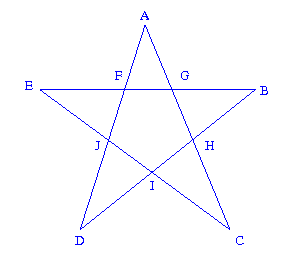
\includegraphics{figures/star}}

\vfill

}

\workbookpagebreak

\item Sketch a graph of the relation 
\[
\{ (x,y) \suchthat x,y \in \Reals \; \mbox{and} \; y > x^2 \}.
\]

\hint{Is this the region above or below the curve $y=x^2$?}

\wbvfill

\item A function $f(x)$ is said to be \index{invertible function} 
\emph{invertible} if there is another function $g(x)$ such that 
$g(f(x)) = x$ for all values of $x$.  (Usually, the inverse function,
$g(x)$ would be denoted $f^{-1}(x)$.)   Suppose a function is presented 
to you as a relation -- that is, you are just given a set of pairs.  
How can you distinguish whether the function represented by this list 
of input/output pairs is invertible?  How can you produce the inverse 
(as a set of ordered pairs)?
 
\hint{If $f$ sends $x$ to $y$, then we want $f^{-1}$ to send $y$ back to $x$.  So the inverse just has the pairs in $f$ reversed.  When is the inverse going to fail to be a function?}

\wbvfill

\workbookpagebreak

\item There is a relation known as ``has color'' which goes from the
set 
\[ F = \{orange, cherry, pumpkin, banana\} \]
to the set 
\[ C = \{orange, red, green, yellow\}. \]

\noindent  What pairs are in ``has color''?
   
\hint{Depending on your personal experience level with fruit there may be different answers.  Certainly
(orange, orange) will be one of the pairs, but (orange, green) happens too!}

\wbvfill

\end{enumerate}



%\newpage
%\renewcommand{\bibname}{References for chapter 1}
%\bibliographystyle{plain}
%\bibliography{main}

%% Emacs customization
%% 
%% Local Variables: ***
%% TeX-master: "GIAM.tex" ***
%% comment-column:0 ***
%% comment-start: "%% "  ***
%% comment-end:"***" ***
%% End: ***

